% Main file for the thesis
% Author: David Pevahouse

\documentclass[a4paper, 11pt]{article}
%------ SETUP OF THE DOCUMENT ------%
%This part of the document sets up the document and makes it easier to read the main.tex file
%------ ********************* ------%
\usepackage[margin = 25mm]{geometry} %
\usepackage{graphicx} % Required for inserting images
\usepackage[toc,page]{appendix}
\usepackage[english=usenglishmax]{hyphsubst} 
\usepackage[hyphens]{url}
\usepackage{amsmath, amssymb, setspace, float, subcaption, caption, booktabs, pdflscape, dcolumn, titlesec, tocloft, comment, xcolor, longtable, blindtext, rotating, lipsum}
\usepackage[flushleft]{threeparttable}
%\usepackage[round, numbers, authoryear]{natbib}
\usepackage[numbers]{natbib}
\usepackage[hidelinks]{hyperref}
\usepackage{array}
\usepackage{multirow}
\usepackage{bashful}


\hypersetup{
     colorlinks   = true, %
     citecolor    = blue, 
     urlcolor = blue, 
    linkcolor = black
}

\graphicspath{{figures/}}

%CHANGE SECTION STYLE
\titleformat{\section}{\normalfont\fontsize{16pt}{20pt}\bfseries}{\thesection}{1.0em}{} %bfseries makes the headings bold
\titleformat{\subsection}{\normalfont\normalsize\bfseries}{\thesubsection}{0.5em}{} %itshape makes the headings in italics
\titleformat{\subsubsection}{\normalfont\normalsize\itshape}{\thesubsubsection}{0.5em}{}

%TABLE OF CONTENTS FIXING
\renewcommand*\contentsname{CONTENTS} %Change name
\setcounter{tocdepth}{2} %How many subsections are visible, 1 is only section headings, 3 include subsubsections

\bibliographystyle{apalike} %closest to LUSEM Harvard referencing guide
\title{Competitive Reinforcement Learning Gaming Agent}
\author{David Pevahouse}
\begin{document}

%THE UNFORTUNATE TITLE PAGE THAT NEEDS TO BE INCLUDED
\setstretch{1.5}



\vspace{2cm}
    \begin{center}       
        \vspace*{2cm}
        {\LARGE {\textbf{Competitive Reinforcement Learning Gaming Agent}}} \\
        \vspace{1cm}
        \Large{David Pevahouse}
    \end{center}
    \vspace{2cm}

\vfill

\thispagestyle{empty}

\newpage
\tableofcontents
\thispagestyle{empty}

\newpage
\maketitle
\begin{abstract}
    Deep reinforcement models in gaming is not entirely new, and in fact has performed quite well on many occasions, with Alphastar being one of the main contenders for high performance\cite{starcraft_unplugged}. This model was capable of overcoming
    99.6 percent of players, achieving one of the highest ranks with both and online and offline Reinforcement learning model. One avenue that has not been explored as deeply however, is using a model to be around the skill level of the opponent providing
    fun and challenging experience to a player regardless of the skill of the player. Most video games today still rely on a typical Easy, Medium, Hard difficulty level which ends up causing problems for both the low end of the spectrum and high end, meaning
    overly difficulty for the bottom players, and to easy for the higher skilled. The goal of this research is to prove the viability of a highly trained Reinforcement Model that's primary objective is not winning but giving a challenge to the opposing agent. This
    paper intends to focus on the novelty of an agent that changes its skill level to challenge its opponent but not to win at every chance.
\setstretch{1}
\end{abstract}
\setcounter{page}{1}

%INTRODUCTION
\hypersetup{linkcolor=blue}
\section{Introduction}
\label{sec:intro}
The background to this idea.

Gaming culture has grown into a phenomenon that has become a part of mainstream culture and it is not at the point where several generations have grown up playing video games. This introduces several problems for game developers. 
The goal of most developers is to create an inviting game that people will enjoy regardless of skill level and competency at video games, at the same time there is a large portion of the community that is skilled and wants a continually increasing 
challenge in their experience. 

In this situation, the word competitive is used to describe the models ability to remain at a skill level close to the player, and not simply the best action to take in a given moment.

One game in specific exemplifies this experience. Starcraft 2 is an real-time strategy game that tests not only the wit of a player or agent, but the ability to outperform physically, in performing as many actions as possible per second that assist in winning
as well as outsmarting their opponent. Obviously this gives the perfect environment for reinforcement learning, and in essence a perfect test for a competitive model that will attempt to match the opponents skill to help ease that learning curve that the genre
of RTS is well known for. 


\subsection{Hypothesis} 
\label{subsec:Hypothesis}
The goal of this research is to test the hypothesis that a trained Model can be competitive rather then just attempting to make the best decisions possible to win. The issues predicted with this is that a model will still need to be as highly trained as a model
capable of beating the best players, but also know game states well enough to not select an action that would crush those players that are not skilled. Typically trained reinforcement learning agents have a cap to the actions they can take, which would end up much 
higher then that of the average person, around 180 actions per minute\cite{vinyals2017starcraft}. Meaning either that has to also scale with player skill, or some actions should be wasted. Either way, the research presented here will be focused on how to design
a model that can compete with a wider skill arrangement then currently available. 

The test here will be to provide an agent that's win ratio against several opponents of differing skill level will be close to 50 percent. This will be tested by training an agent then having it compete against several opponents trying to obtain around 50 percent
win ratio regardless of opponent over a course of 50 games. The rationale behind this, is that if an agent is truly competitive and not purely trying to win, then it should lose about the same amount as it wins to provide an experience of learning and improving
with a human player regardless of skill. 


\subsection{Theory} 
\label{subsec:Theory}
Typically a model follows being trained on an environment and selecting the best possible action given the current state of the game. The problem with that philosophy in this situation is that the player agent may not be taking the best possible action. In order
to give the player a chance to compete and be challenged, the theory is that the model should select the "average" action. In order to have an average action that is still competitive to any player, that model must still be capable of performing the best possible
action. This is both a boon and a curse, in theory. That means the training of a model should be the exact same, but instead of selecting the highest scoring action, the model should select the lowest absolute value, on a normal scale of reward being from -1 to 1. 
If it selects the reward of closest to zero, the lowest absolute value, in theory that action would be the most likely to lead to a tie. Since games in Starcraft 2 rarely end up in a tie, in theory this means that it will be a close game. 

Other theories to go with the hypothesis that will be tested to add to the novelty of how this agent is being piloted, will be not just selecting the closest value to 0, not positive or negative, in the model, but also checking out other possible options, such As
half the best, three quarters the best, and the second best to see how the agent performs with those actions.
%PREVIOUS LITERATURE
\section{Previous Research}
\label{sec:Previous Research}
As previously mentioned, Starcraft 2 has been a prime target for previous research in the field of Reinforcement learning with plenty of sources diving into trying to create the best model\cite{starcraft_unplugged}\cite{liu2021mAS}\cite{liu2021mASreport}\cite{vinyals2017starcraft}.
These typically focused on a specific component of this problem, which there are many. Pysc2 was created to give an environment for the community to collectively access the games controls quickly and efficiently, which sets up the environment and state for 
reinforcement learning\cite{vinyals2017starcraft}, which will be used in this research and explained further later on. This placed the ground work for the most successful model in Starcraft 2 to day, Alphastar\cite{starcraft_unplugged} using both offline and
online learning and providing a good ceiling for what is capable. While Alphastar was developed by a team of highly skilled developers, and plenty of hardware to train that is not available to everyone, which using a lighter weight model\cite{liu2021mASreport}.
This was further expanded in creating a version not tied to being trained on specific replays while continuing to be light weight\cite{Liu2022OnER}. 

All this to show that Starcraft 2 is rich for the exploration of the world of Reinforcement learning, due to the difficulty of the problem which will be expanded upon later. To build upon this research is a tall task, but the goal is to take it to the next level
to be used practically by not just Starcraft 2, but potentially take the concepts and apply to any game for a scaling and competitive difficulty to be applicable to a much larger range of players. 

Other research centered around the idea of a changing difficulty agent is a thesis from Robin Lievrouw, centered around single player Dynamic Difficulty Adjusting (DDA)\cite{lievrouw_applying_2020}. Here there was an extensive study done on the game Space Invaders by 
determining instead of an easy, medium, hard, difficulty range if these were less hard and fast rules but more fluctuating between a beginner reinforcement learning, to an advance. There was a study done by humans in determining satisfaction and along with that
the average Q level of these models as they were not aiming for the highest result in this specific example. 

However, this case is more similar to a report done at the Institute of Electronics and Informatics Engineering of Aveiro from the University of Aveiro\cite{reis_automatic_2023}. This study takes it to the next level, and was shown at the IEEE 2023 Conference of 
Games. The focus here is instead of DDA, taking it to multiplayer dynamic difficulty adjusting (MDDA). The difference is slight but does matter. The goal of DDA was for single player games making the environment of the game be flexible with the difficulty in scaling to 
the player, whereas MDDA focuses on games where the opponents are other players so it would be an RL agent as the opposing player. This sounds easier at first due to limiting it to an agent instead of an environment, but the difficulty comes with the agent having
the same decisions as a player does which happens to be extensive as this research will show later. 
%BACKGROUND
\section{Environment and Agent}
\label{sec:Environment and Agent}

The environment for Starcraft 2 to is notoriously complicated, where taken at its raw value the action space would have up to $10^{26}$ per step. Obviously that is computationally to expensive, so there was an environment developed to limit the steps possible. This
can be done with several different thought process combined. One, not all actions that are possible for a given state, are possible for every given state. For example, training a marine without the barracks selected, or even without a barracks built. So that 
can limit action spaces. Another limitation is to combine certain actions, for example selecting marines and attack-moving the units to a different location as a single action instead of 3-4 or more. This is done by reducing actions a using an auto-regressive
chain rule to limit the action space given the context above\cite{starcraft_unplugged}: $$\pi_{\theta}(a|s) = \prod\limits_{l=0}^{L} \pi_{\theta}(a^l|a^{<l}, s)$$.

Another key component to the environment is that Starcraft is an incomplete information game, meaning that there is limited information on the model at any given time, so part of the action space and model needs to learn how to explore and make decision with
incomplete information. 

The agents often have to make use of learning the actions provided in the environment, especially with the capability of so many actions being available at once in the policy. The learning algorithm with seemingly the best results, according to the creators of
pysc2 is, in order of policy gradient, value estimation gradient, and entropy regularisation: 
$$\underbrace{(G_t - v_\theta(s_t))  \nabla_\theta \log \pi_\theta(a_t|s_t)} + \beta \underbrace{(G_t - v\theta(s_t)) \nabla_\theta v_\theta(s_t)} + \eta \underbrace{\sum_a \pi\theta(a|s_t) \log \pi_\theta(a|s_t)}, \qquad (1)$$

While these are the two major equations that go into this environment and recommended agent, they are not the only ones and for more details, refer to the original cited papers. The goal of the agent here is not to match the performance of the previous research
but take the idea of RL in Starcraft II and games in general and aim for a model that can challenge any player, but not aim to win rather then just be challenging.
\subsection{Experiment Details}

With this in mind, the intention of this experiment is not to have the most accomplished Starcraft Model. There have been teams of people, each much more accomplished then myself working on that, but instead to create a model that can fluctuate its
skill with the state of the game. This agent and environment will be run on a machine leaning towards the weak side, running an Nvidia 2070 GPU, 32gbs of ram, and an Intel I7. Tests were run on two machines with the only difference being a 6th gen I7 vs a 10th gen.
These limitations prevents a few advanced features such as using several models to categorize actions with a selection model to chose which action category to take, this experiment will only be using a singular model. Another advanced feature that would in theory
be beneficial for this experiment is to train and use computer vision on replays of professional Starcraft II players, but again due to constraints this will be a simple pure reinforcement learning model. Lastly, the environment will be stripped down, from the
aformentioned details above, with the constraints previously mentioned, a pure environment cannot be used. Instead, it is stripped to 21 different states based on the resources, whats been built, and what units are available. From that state, there are 6 possible
actions. These actions are: do nothing, build supply depot, build barracks, train marines, and attack.  To train, the environment will consist of one agent and a random agent, the experiment will be similar except the opposing agent will differ. Below is an 
image from the environment running.

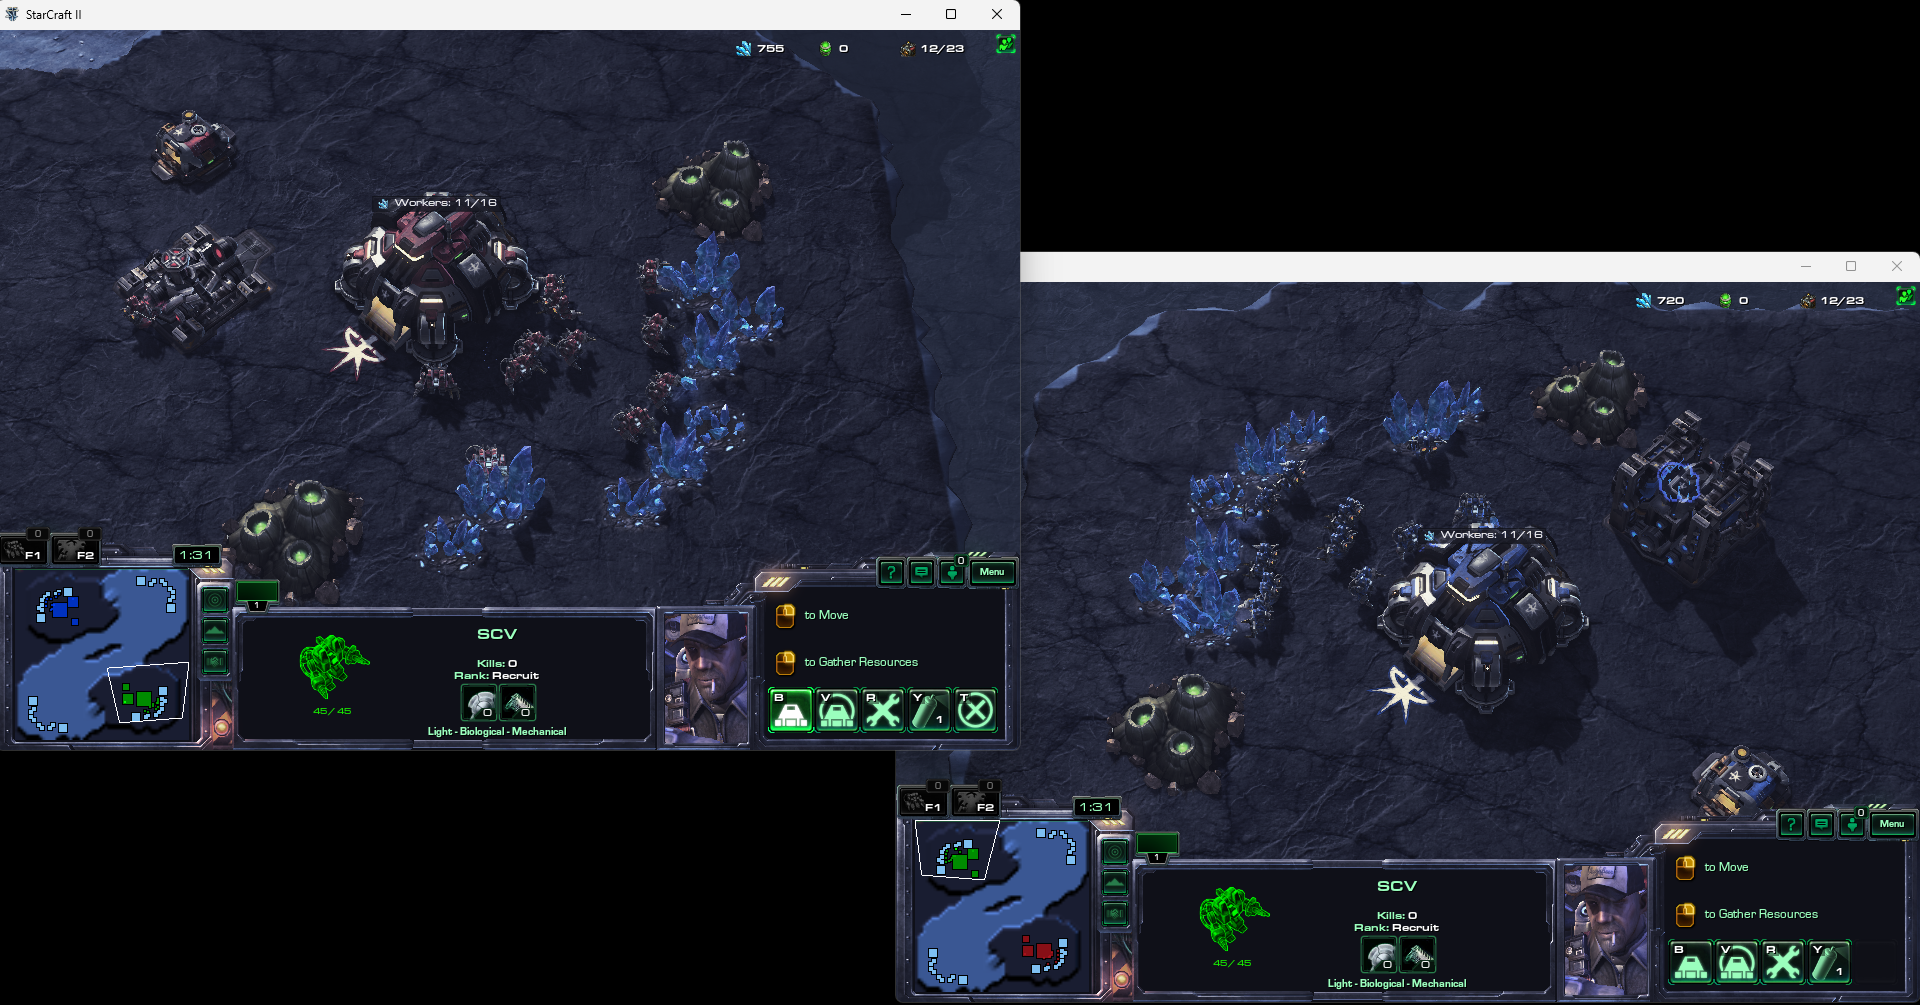
\includegraphics[width=.5\textwidth]{images/sc2env.png}
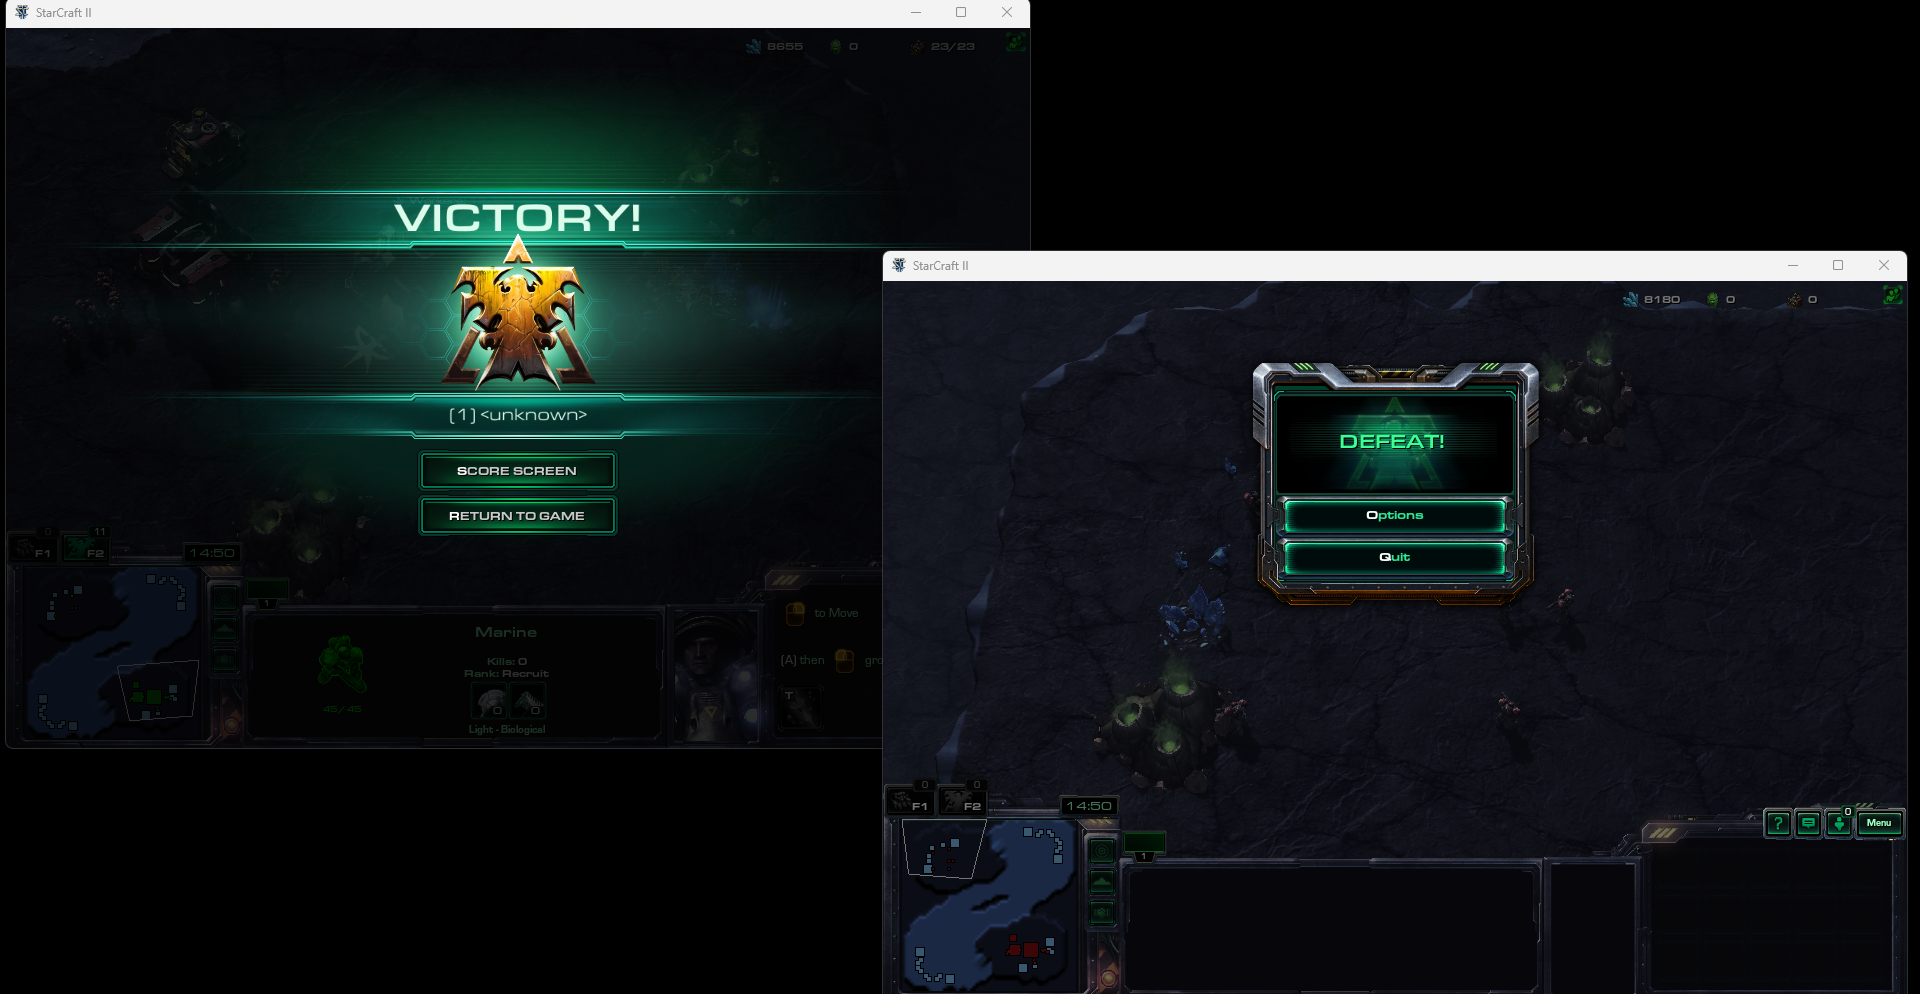
\includegraphics[width=.5\textwidth]{images/victory_screen.png}

\subsection{Agent Details}
Due to the shrunken environment the agents will be fairly limited in their capability as this is not a fully fledged game of Starcraft II. There will be three primary agents in it however, and two are modified to perform this experiment. First, a Q Learning
agent (QL). This is meant to be a reliable, strong, but not perfect model. The adjustments made in order to test the hypothesis have several modes to see what is most likely to give the end goal. There are five action types, normal or none, neutral action to grab
the action in the middle, second for the second best action, quarter for the third-quarter best action, and half best for the half best positive action. Then in addition to that change, in order to implement further tests, there is an alternating variable
to incorporate experiment. Essentially this change has the models action selection alternate from the previous adjustments mention, and the best action that is typical. In essence making half the decisions the best decisions possible, and the other half the 
specified test The second model is a Deep Q Learning agent (DQN). The agent has been implemented with 2 networks in order to stabilize and regularize the agent as it learns. There needs to be a disclaimer with this experiment using these agents. 
Since the environment is simplistic as it is, there could be a missed opportunity to truly test the potential of these changes. More information will be described in future work.

This means that the experiment will be run this way. A player one will be selected from the DQN and QL model. Next a player two will be selected from DQN, QL, and random agent. Player one will have a combination of alternation between the competitive level 
variable, or not, and the combination variable determining the test. As it has been said before, this experiment is not focused on a perfect model, others have done that. The novelty of this experiment is to make a model that can adjust its difficulty based 
on the skill of the opponent, and with three levels of agents here, the experiment should should any measure of success in the theory. 
%DATA
\section{Training Methodology}
\label{sec:Training Methodology}


There are multiple differing methods to training a model, from offline to online, meaning a model that is fully trained and ready to compete vs a model that is learning as it goes and continues to update. Currently the highest performing model is trained in an
offline manner on hundreds of thousands of replays\cite{starcraft_unplugged}. Unfortunately, that method is not plausible given the current time and computational restraints, so a more efficient model based on online training will be used as a proof of concept. 
Even so, this will not be an easy task to replicate as the computational expense is far to high, so the proof of concept will be limited. The model that will be the basis of testing uses a hierarchical architecture to learn and solve problems without a usage offline
raw data and human replays, such as Alphastar, that in some ways eliminate the true intention of reinforcement learning, even if it does solve the problem\cite{Liu2022OnER}.

That makes the Alphastar method unlike how a human would play the game, and creates issues since Starcraft 2 replays are only playable on the patch it was created at, and there other methods to get around this. This experiment will be closer to a true reinforcement
learning methodology here, though limited. One important distinction to make in this experiment however, is even when there is the capability of fluctuating skill level against a player, in the training process that is not being saved. The model needs to know how 
to perform at the best of its capabilities regardless of the opponent, which means it would need to be capable of performing at best, as well as fluctuating to lower levels.

\subsection{Games}
In order to train the agents, both will be trained over 1000 games versus a random agent. The games will be run at 128 times the normal speed, otherwise this would take days or weeks. Pysc2 works by expecting agents to have a step method to make a decisions 
move to the next frame of the game. There is also the stipulation that the game will not last longer then 20 minutes. This is to prevent an agent from getting itself into a position where it cannot lose and just staying in place. Rewards also have to be determined
due to how the game works. So winning is associated with a 1, a tie is associated with 0, and a loss as -1. These have to be propagated into the actions to determine how successful they are. Then the agent and the models associated need a strategy to learn.

Rewards here are determined by Starcraft II api that pysc2 pulls that is based on a combination of resources gathered, units trained, buildings built, and units killed. \cite{vinyals2017starcraft}


\subsection{Parameters and Learning}
To deal with the problem of an agent choosing to focus on tieing, due to that being an easier goal to reach, there has to be an element of randomness and a reduction in the rewards being received to accurately reduce some actions having more weight. For example,
training an army of marines at the base but never attacking would lead to a tie every time and guarantee some level of rewards. A level of randomness, exploration, needs to be added to further decrease the odds of that happening. The DQN was specifically prone to
the issue of always tying, as a few things would have such a high weighted action. To combat it in the DQN specifically, there is, in additional step to increment epsilon, allowing it to change and fluctuate, some episodes would have a high epsilon causing 
exploration to take priority over exploitation, and vise versa, so that actions later in the game would be weighted as well. 

This also requires careful tuning of the learning rate, and surprisingly batch size with a replay buffer. For training purposes, the replay buffer holds a history of the steps of the game for DQN, and the batch size determines how many of that replay buffer will
be used for training. This can add significant randomness due to the level of steps that need to be recorded, as it could train on, for example, 256 steps that all recorded do nothing, which as to our previous example, can lead to after building an army, to not 
attack. This makes both batch size for training, and maximum replay buffer to see how long to hold steps other parameters to determine learning. 

\section{Results}
\label{sec:results}

To proceed into the experiments, the methodology of test will have the trained models, DQN and RL, perform a series of test between alternating the competitive selection between the variable the normal best, and then the specific competitive variable, and the same
competitive variable without alternation per trained model. This was by playing 50 episodes/games against each opponent, for example a DQN with alternating and neutral competitive versus a normal DQN, QL, or random. To provide a baseline of which is better, DQN or 
QL in this situation based on the training they received, the below chart are those two head to head.

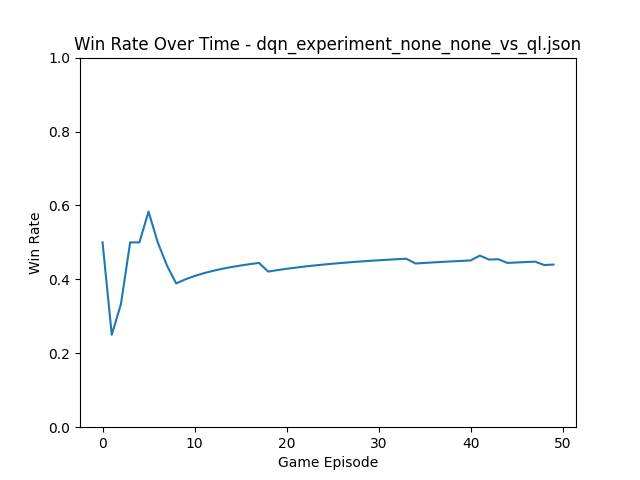
\includegraphics[width=0.5\textwidth]{images/win_rate_dqn_experiment_none_none_vs_ql.png}

From this baseline it can be seen that the DQN and the QL model perform around the same level, and looking into the statistics themselves of their competition nearly every game was a stalemate with only a few games where one conquered the other. 

\subsection{Data}

To clarify what the below charts mean by win rate, a win consists of a 1, a loss, 0, but since a tie in essence is also an desirable state considering that would mean it is challenging enough to not lose, but scales to the difficulty to not win as well, a tie
adds .5 to the win ratio, meaning that if a model tied every single game it would achieve a desirable 50 percent win ratio. This does slightly skew the results due to that caveat but the results it produces are beneficial for this experiment specifically. 
In addition, there is more information available that includes total rewards and a moving average reward included in the Appendix A, but for the sake of readability it was not included here.

\begin{tabular}{>{\centering\arraybackslash}m{0.05\textwidth}>{\centering\arraybackslash}m{0.3\textwidth}>{\centering\arraybackslash}m{0.25\textwidth}>{\centering\arraybackslash}m{0.25\textwidth}}
    & \multicolumn{3}{c}{\textbf{DQN without Alternating}} \\
    & \textbf{Vs Random} & \textbf{Vs QL} & \textbf{Vs DQN} \\
    \textbf{Neutral} & 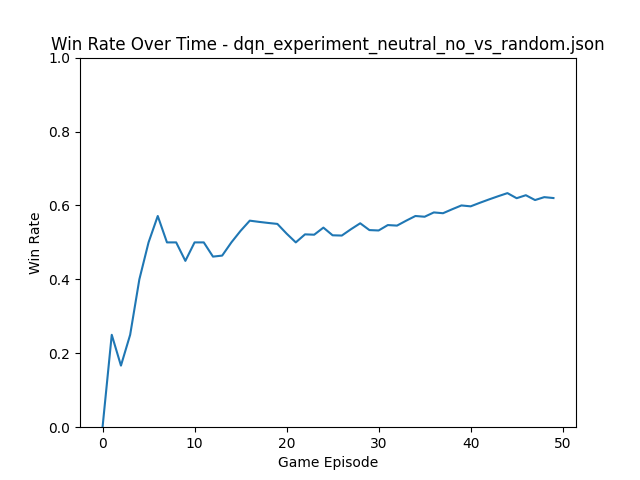
\includegraphics[width=0.25\textwidth]{images/win_rate_dqn_experiment_neutral_no_vs_random.png} &
    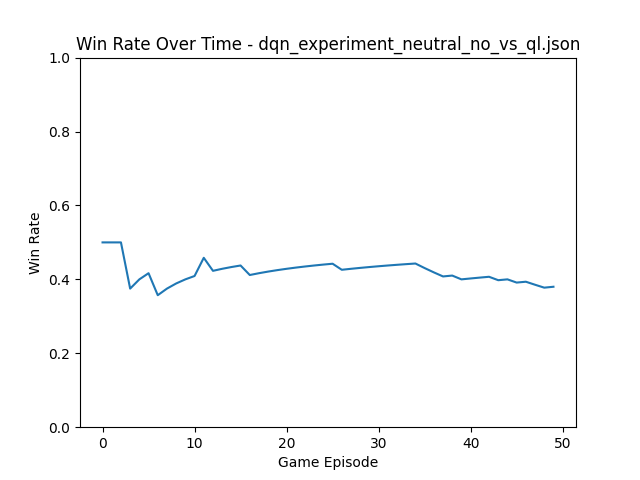
\includegraphics[width=0.25\textwidth]{images/win_rate_dqn_experiment_neutral_no_vs_ql.png} &
    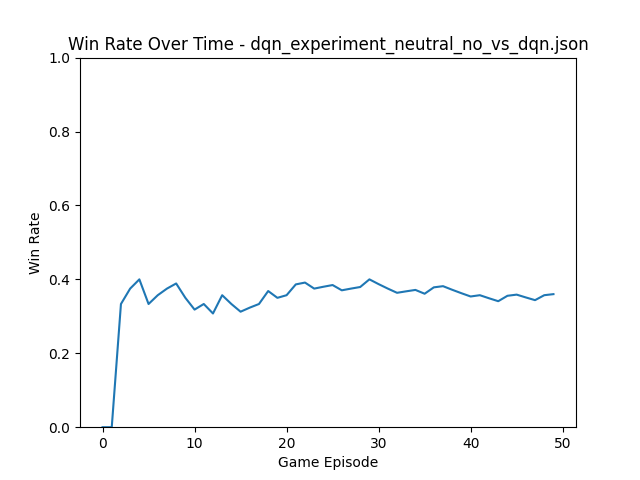
\includegraphics[width=0.25\textwidth]{images/win_rate_dqn_experiment_neutral_no_vs_dqn.png} \\
    \textbf{Half} &  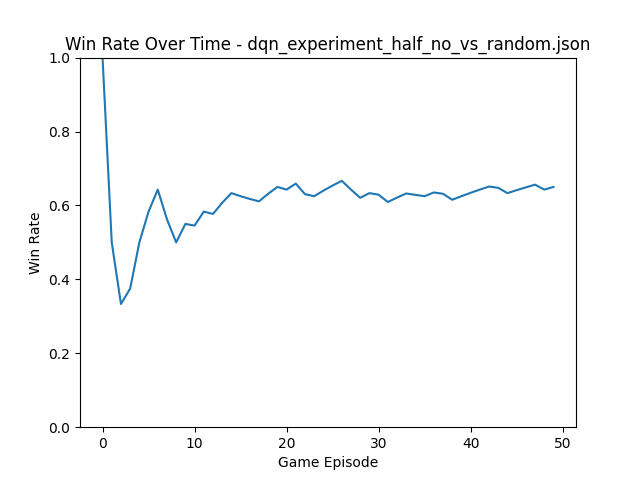
\includegraphics[width=0.25\textwidth]{images/win_rate_dqn_experiment_half_no_vs_random.png} & 
    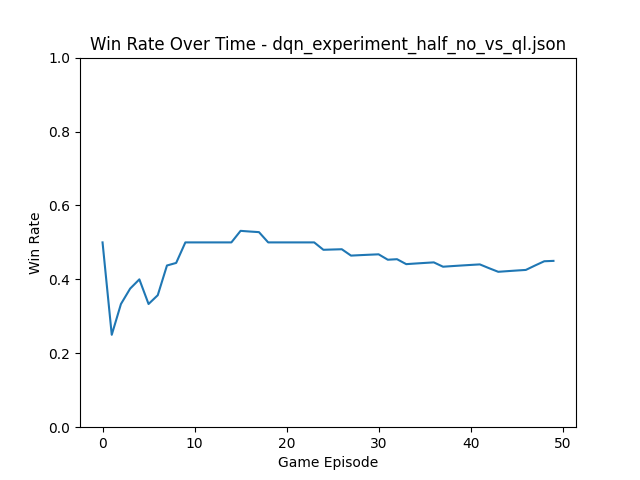
\includegraphics[width=0.25\textwidth]{images/win_rate_dqn_experiment_half_no_vs_ql.png} &
    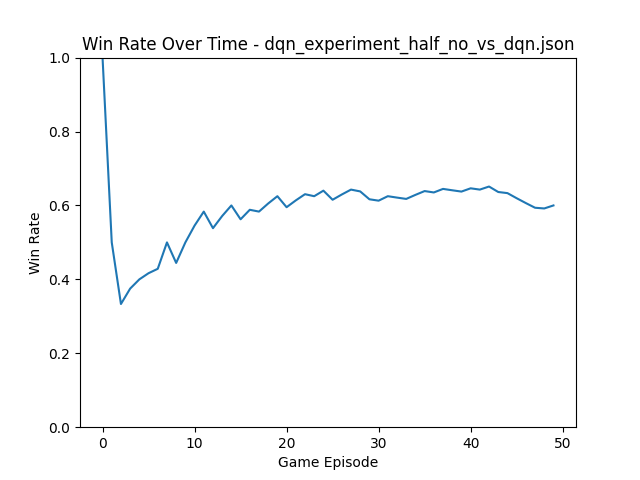
\includegraphics[width=0.25\textwidth]{images/win_rate_dqn_experiment_half_no_vs_dqn.png} \\
    \textbf{Quarter} & 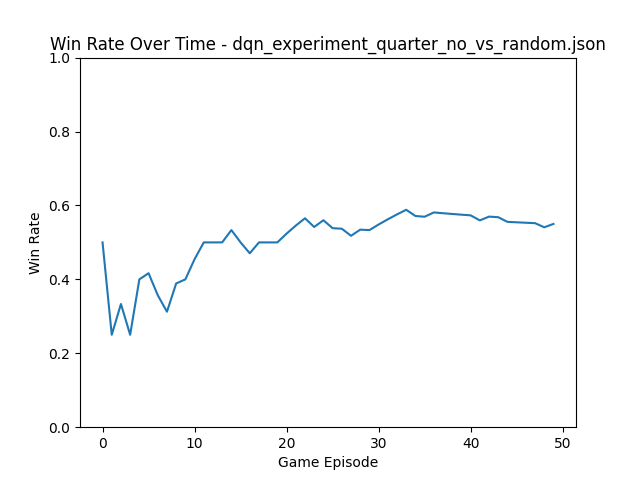
\includegraphics[width=0.25\textwidth]{images/win_rate_dqn_experiment_quarter_no_vs_random.png} &
    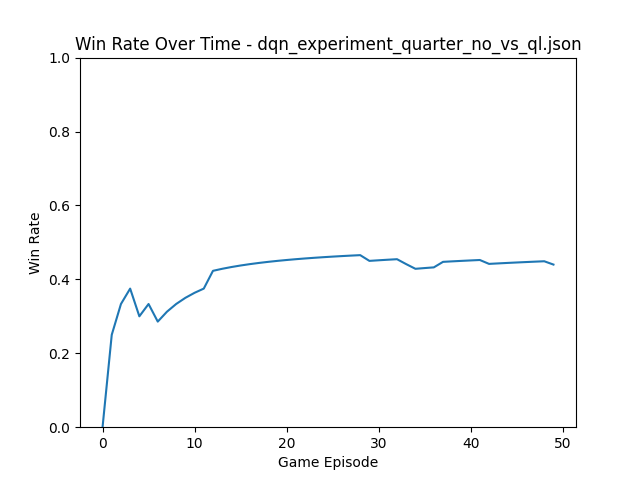
\includegraphics[width=0.25\textwidth]{images/win_rate_dqn_experiment_quarter_no_vs_ql.png} &
    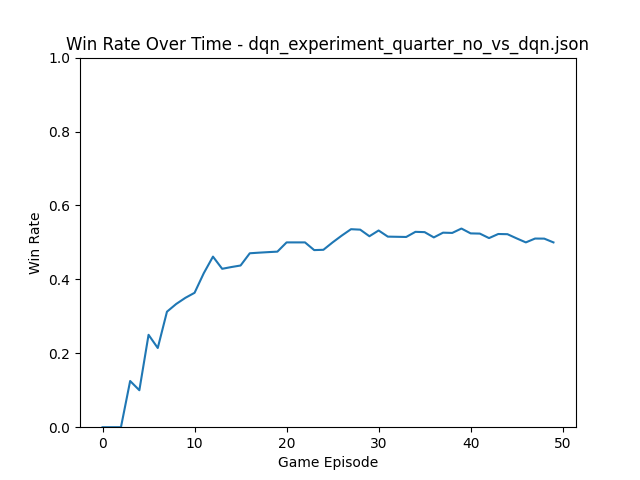
\includegraphics[width=0.25\textwidth]{images/win_rate_dqn_experiment_quarter_no_vs_dqn.png} \\
    \textbf{Second} & 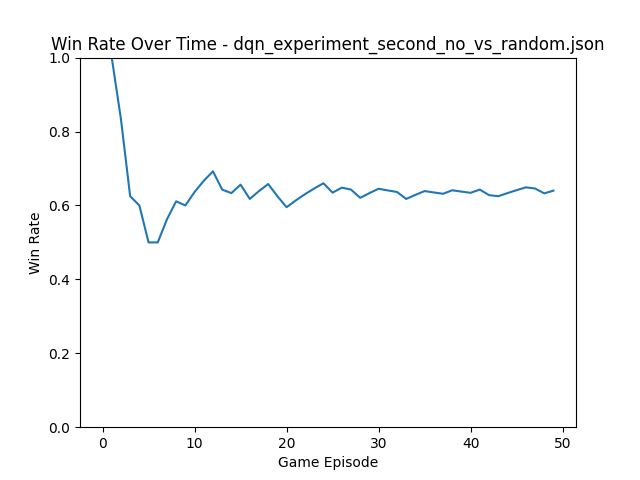
\includegraphics[width=0.25\textwidth]{images/win_rate_dqn_experiment_second_no_vs_random.png} &
    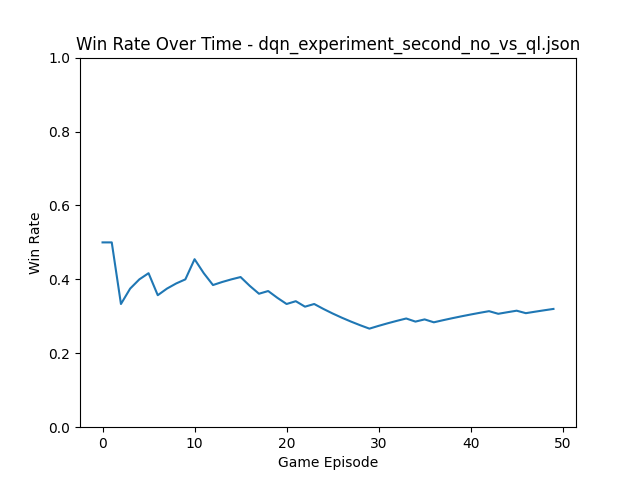
\includegraphics[width=0.25\textwidth]{images/win_rate_dqn_experiment_second_no_vs_ql.png} &
    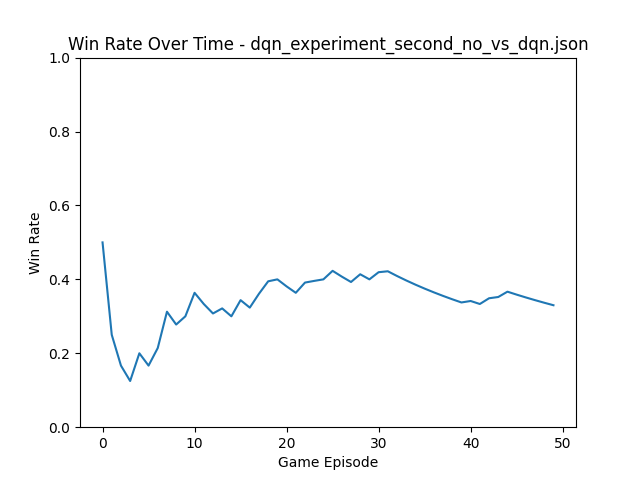
\includegraphics[width=0.25\textwidth]{images/win_rate_dqn_experiment_second_no_vs_dqn.png} \\
  \end{tabular}

  \begin{tabular}{>{\centering\arraybackslash}m{0.05\textwidth}>{\centering\arraybackslash}m{0.3\textwidth}>{\centering\arraybackslash}m{0.25\textwidth}>{\centering\arraybackslash}m{0.25\textwidth}}
    & \multicolumn{3}{c}{\textbf{DQN with Alternating}} \\
    & \textbf{Vs Random} & \textbf{Vs QL} & \textbf{Vs DQN} \\
    \textbf{Neutral} & 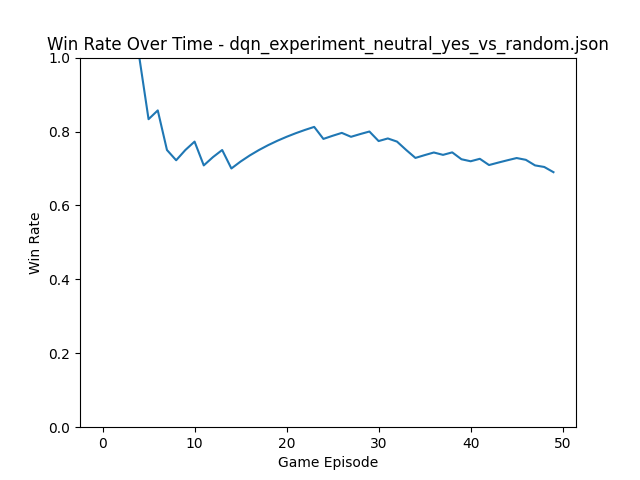
\includegraphics[width=0.25\textwidth]{images/win_rate_dqn_experiment_neutral_yes_vs_random.png} &
    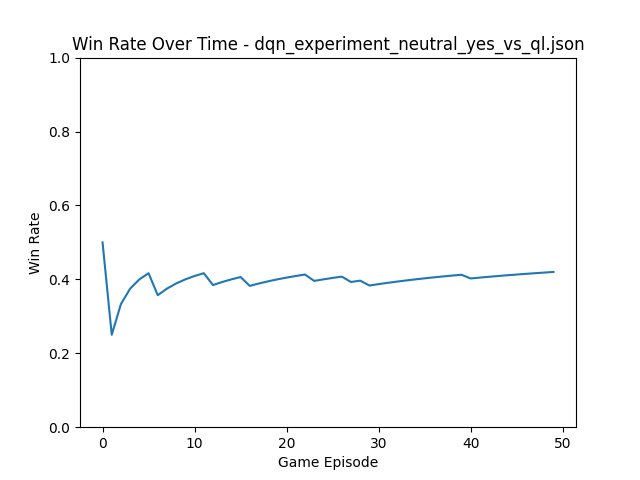
\includegraphics[width=0.25\textwidth]{images/win_rate_dqn_experiment_neutral_yes_vs_ql.png} &
    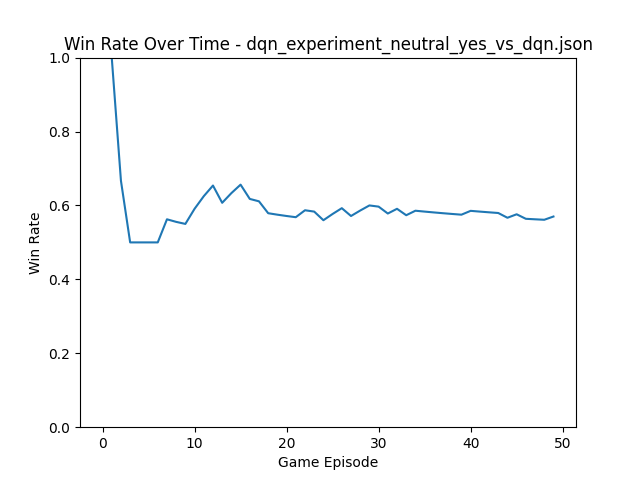
\includegraphics[width=0.25\textwidth]{images/win_rate_dqn_experiment_neutral_yes_vs_dqn.png} \\
    \textbf{Half} &  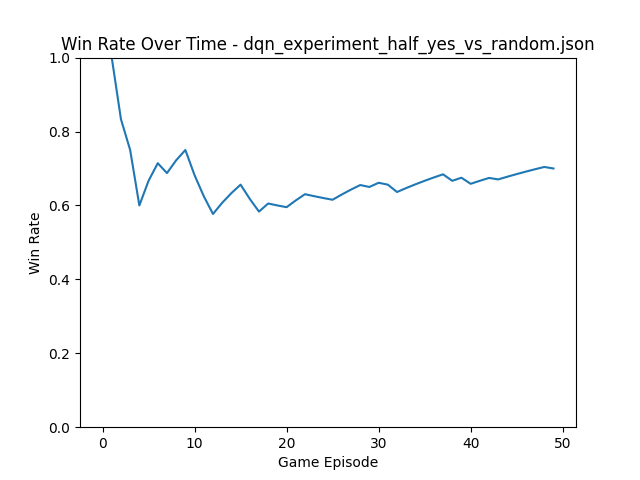
\includegraphics[width=0.25\textwidth]{images/win_rate_dqn_experiment_half_yes_vs_random.png} & 
    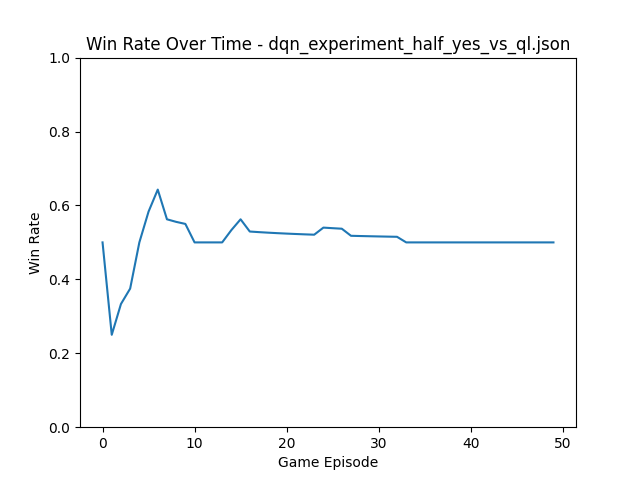
\includegraphics[width=0.25\textwidth]{images/win_rate_dqn_experiment_half_yes_vs_ql.png} &
    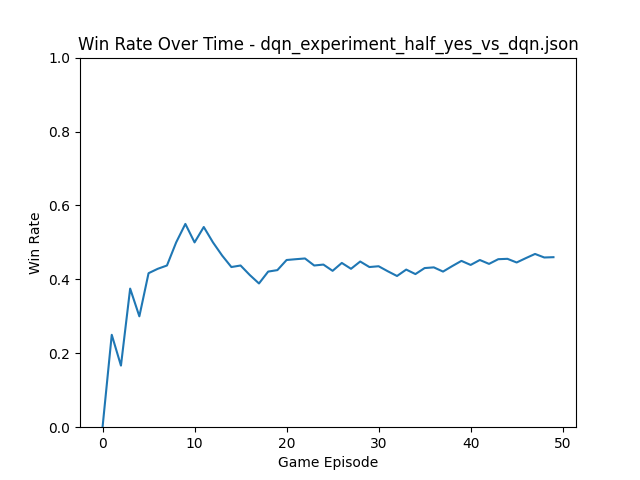
\includegraphics[width=0.25\textwidth]{images/win_rate_dqn_experiment_half_yes_vs_dqn.png} \\
    \textbf{Quarter} & 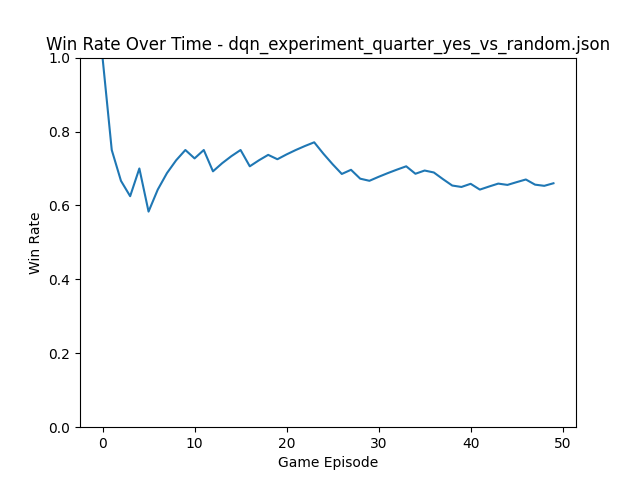
\includegraphics[width=0.25\textwidth]{images/win_rate_dqn_experiment_quarter_yes_vs_random.png} &
    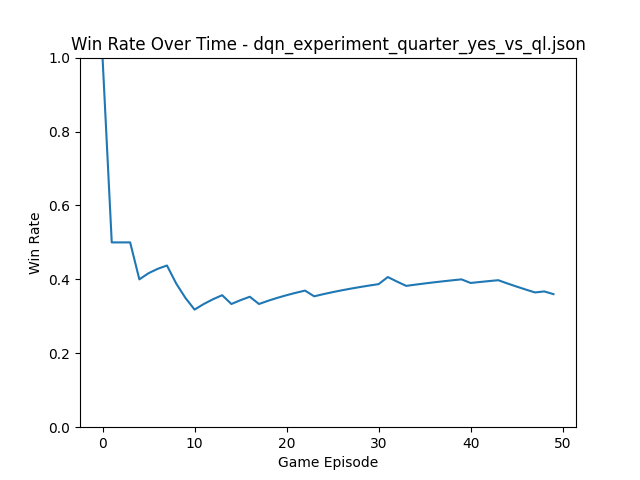
\includegraphics[width=0.25\textwidth]{images/win_rate_dqn_experiment_quarter_yes_vs_ql.png} &
    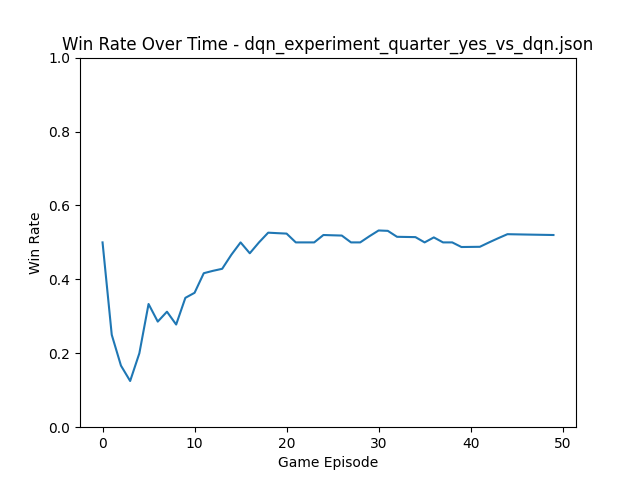
\includegraphics[width=0.25\textwidth]{images/win_rate_dqn_experiment_quarter_yes_vs_dqn.png} \\
    \textbf{Second} & 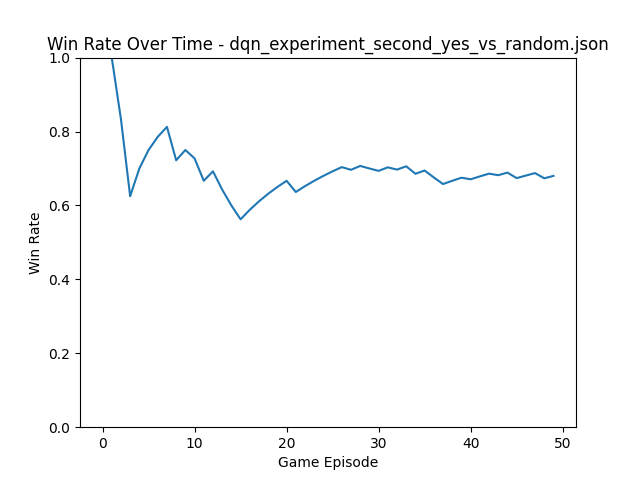
\includegraphics[width=0.25\textwidth]{images/win_rate_dqn_experiment_second_yes_vs_random.png} &
    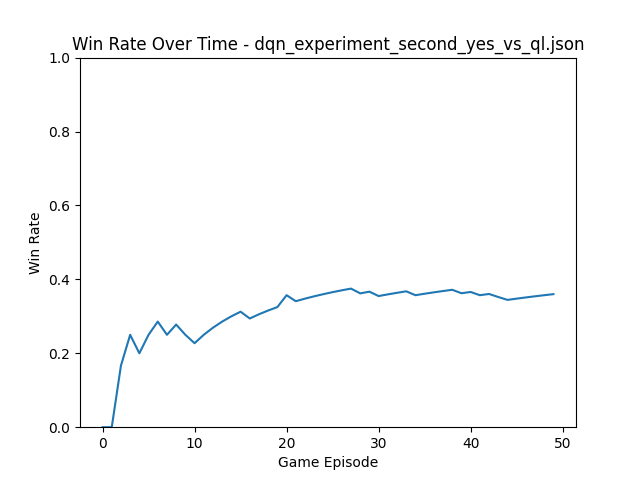
\includegraphics[width=0.25\textwidth]{images/win_rate_dqn_experiment_second_yes_vs_ql.png} &
    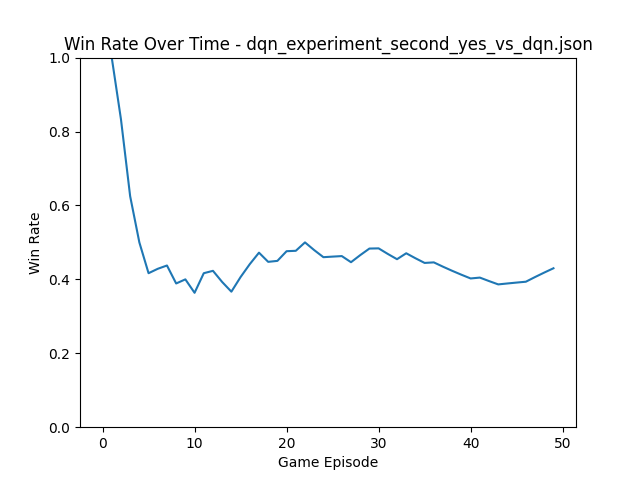
\includegraphics[width=0.25\textwidth]{images/win_rate_dqn_experiment_second_yes_vs_dqn.png} \\
  \end{tabular}

  \begin{tabular}{>{\centering\arraybackslash}m{0.05\textwidth}>{\centering\arraybackslash}m{0.3\textwidth}>{\centering\arraybackslash}m{0.25\textwidth}>{\centering\arraybackslash}m{0.25\textwidth}}
    & \multicolumn{3}{c}{\textbf{QL without Alternating}} \\
    & \textbf{Vs Random} & \textbf{Vs QL} & \textbf{Vs DQN} \\
    \textbf{Neutral} & 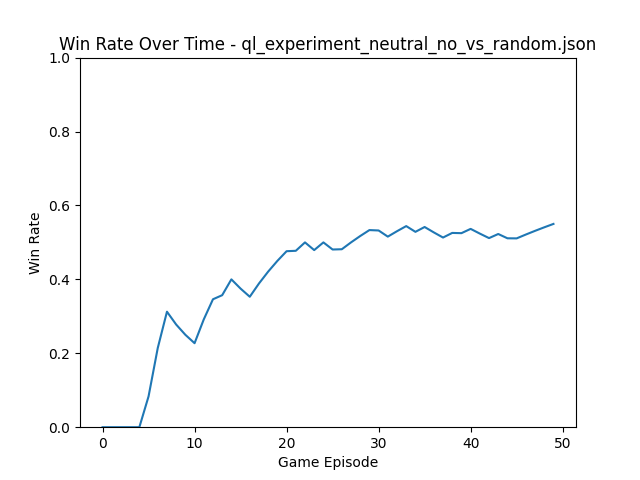
\includegraphics[width=0.25\textwidth]{images/win_rate_ql_experiment_neutral_no_vs_random.png} &
    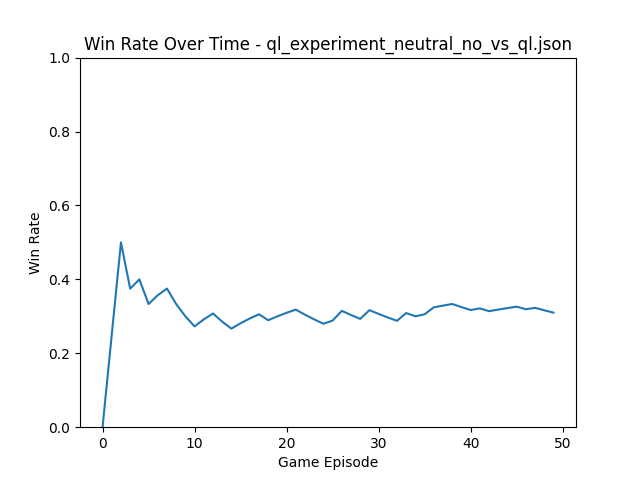
\includegraphics[width=0.25\textwidth]{images/win_rate_ql_experiment_neutral_no_vs_ql.png} &
    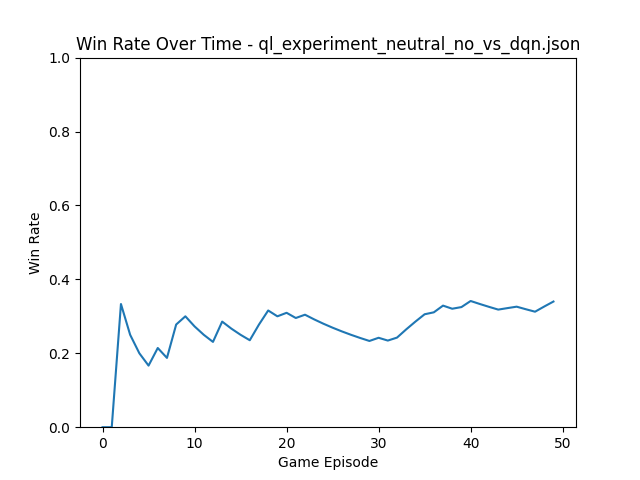
\includegraphics[width=0.25\textwidth]{images/win_rate_ql_experiment_neutral_no_vs_dqn.png} \\
    \textbf{Half} &  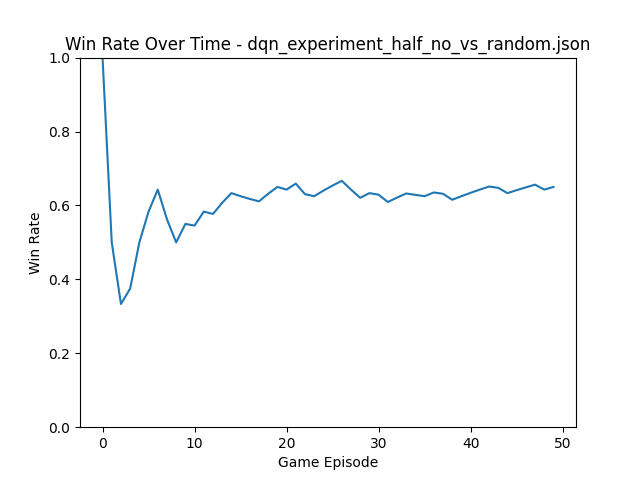
\includegraphics[width=0.25\textwidth]{images/win_rate_dqn_experiment_half_no_vs_random.png} & 
    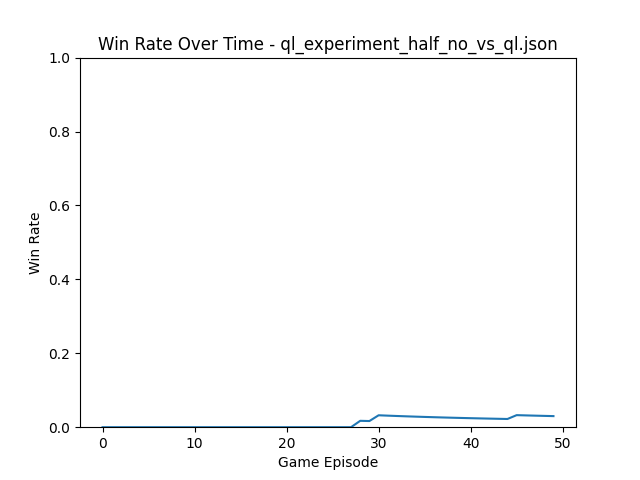
\includegraphics[width=0.25\textwidth]{images/win_rate_ql_experiment_half_no_vs_ql.png} &
    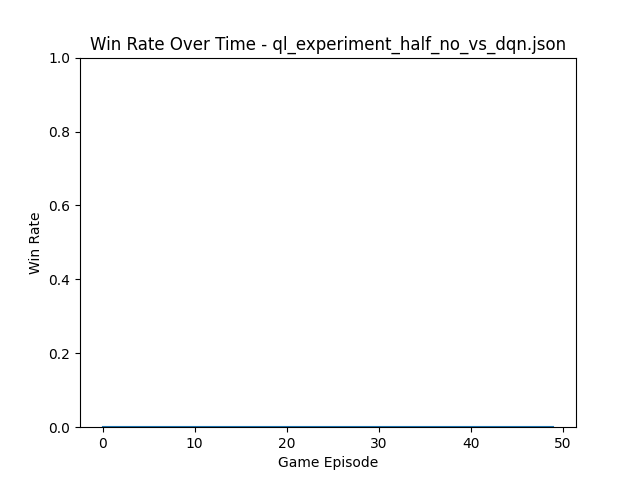
\includegraphics[width=0.25\textwidth]{images/win_rate_ql_experiment_half_no_vs_dqn.png} \\
    \textbf{Quarter} & 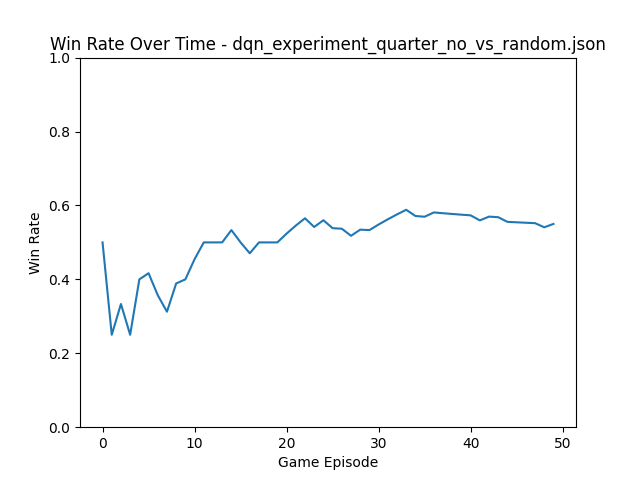
\includegraphics[width=0.25\textwidth]{images/win_rate_dqn_experiment_quarter_no_vs_random.png} &
    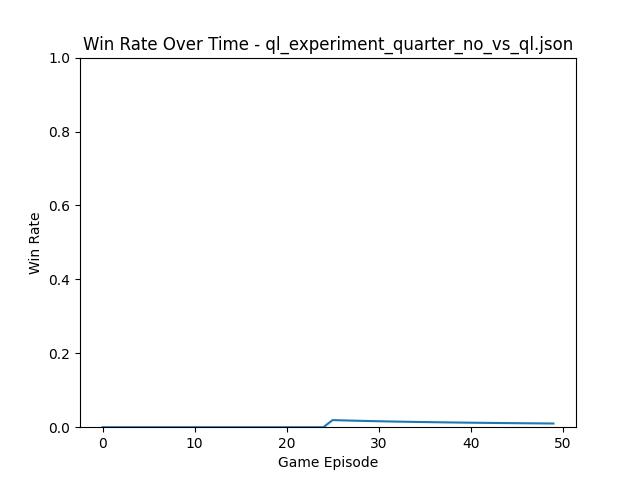
\includegraphics[width=0.25\textwidth]{images/win_rate_ql_experiment_quarter_no_vs_ql.png} &
    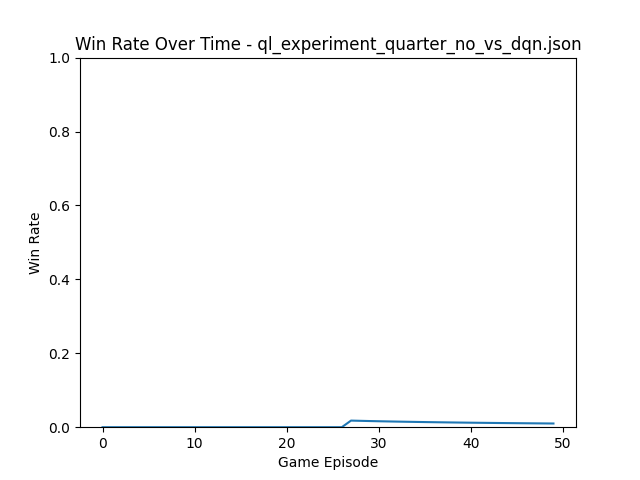
\includegraphics[width=0.25\textwidth]{images/win_rate_ql_experiment_quarter_no_vs_dqn.png} \\
    \textbf{Second} & 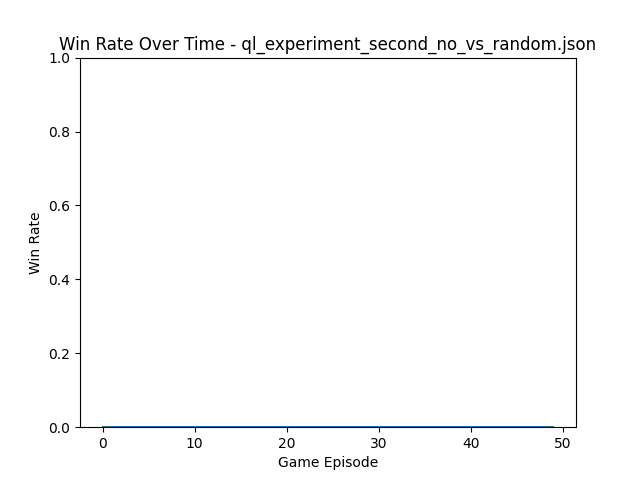
\includegraphics[width=0.25\textwidth]{images/win_rate_ql_experiment_second_no_vs_random.png} &
    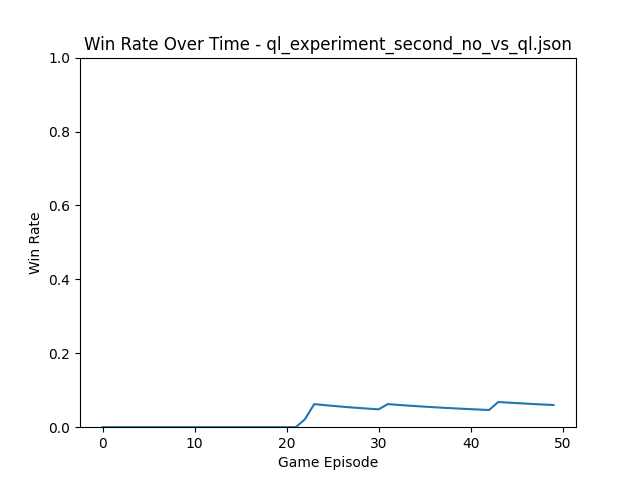
\includegraphics[width=0.25\textwidth]{images/win_rate_ql_experiment_second_no_vs_ql.png} &
    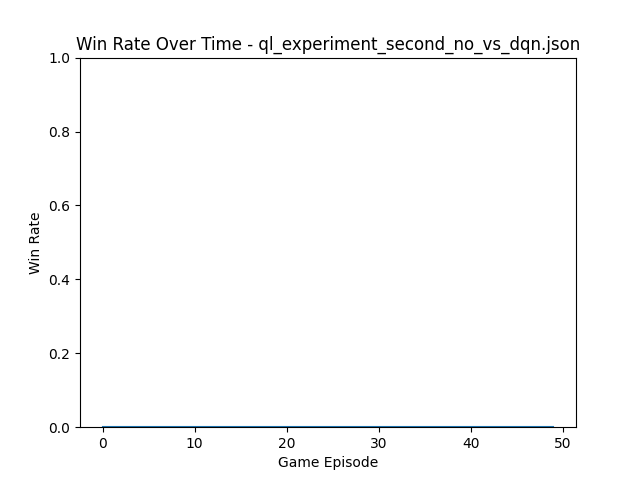
\includegraphics[width=0.25\textwidth]{images/win_rate_ql_experiment_second_no_vs_dqn.png} \\
  \end{tabular}

  \begin{tabular}{>{\centering\arraybackslash}m{0.05\textwidth}>{\centering\arraybackslash}m{0.3\textwidth}>{\centering\arraybackslash}m{0.25\textwidth}>{\centering\arraybackslash}m{0.25\textwidth}}
    & \multicolumn{3}{c}{\textbf{QL with Alternating}} \\
    & \textbf{Vs Random} & \textbf{Vs QL} & \textbf{Vs DQN} \\
    \textbf{Neutral} & 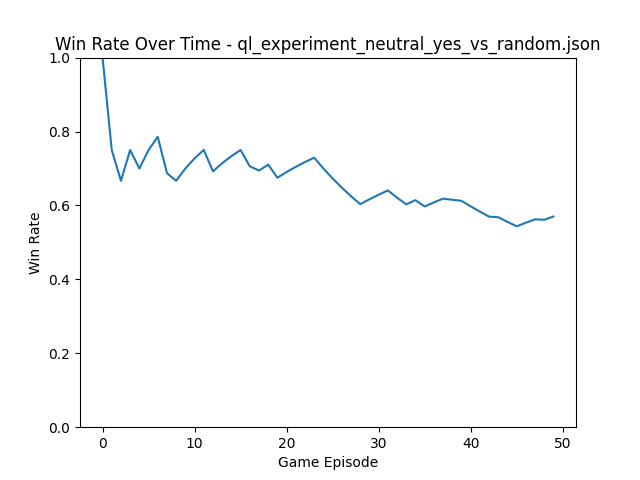
\includegraphics[width=0.25\textwidth]{images/win_rate_ql_experiment_neutral_yes_vs_random.png} &
    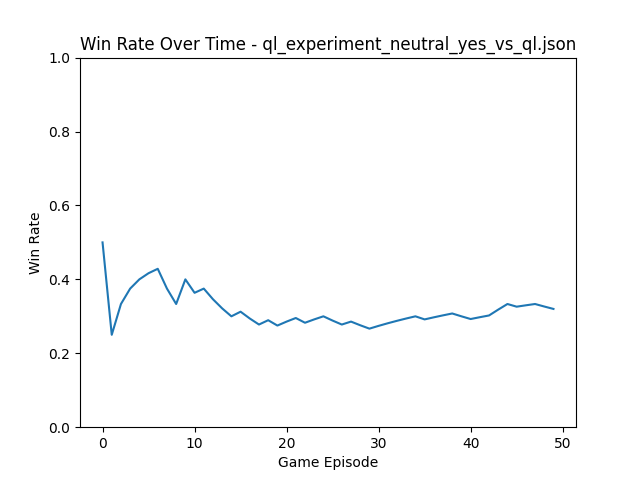
\includegraphics[width=0.25\textwidth]{images/win_rate_ql_experiment_neutral_yes_vs_ql.png} &
    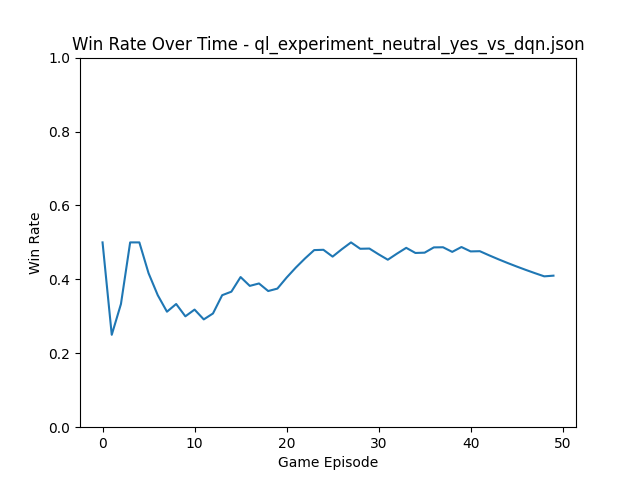
\includegraphics[width=0.25\textwidth]{images/win_rate_ql_experiment_neutral_yes_vs_dqn.png} \\
    \textbf{Half} &  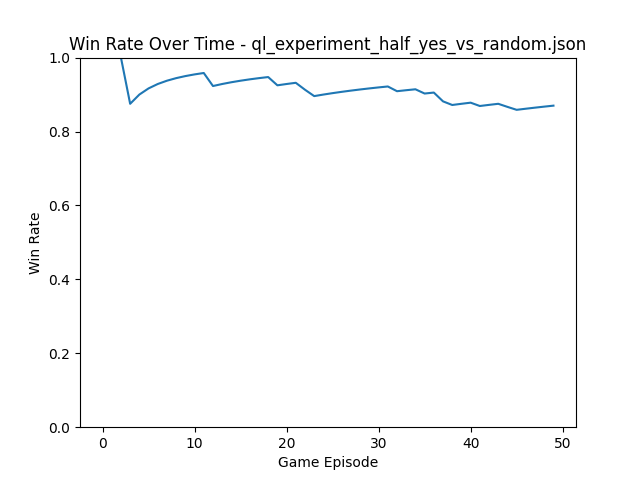
\includegraphics[width=0.25\textwidth]{images/win_rate_ql_experiment_half_yes_vs_random.png} & 
    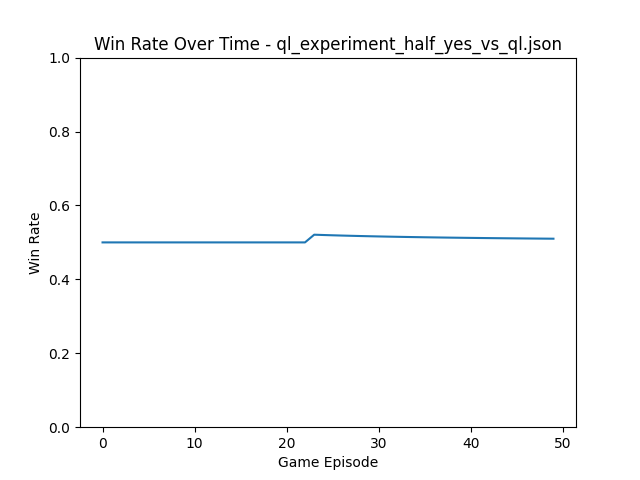
\includegraphics[width=0.25\textwidth]{images/win_rate_ql_experiment_half_yes_vs_ql.png} &
    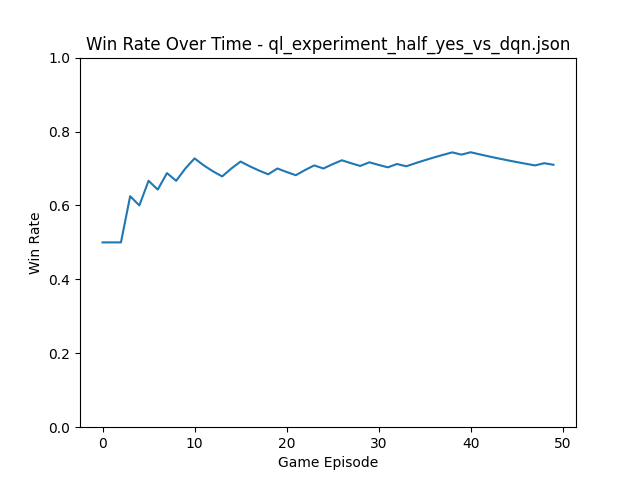
\includegraphics[width=0.25\textwidth]{images/win_rate_ql_experiment_half_yes_vs_dqn.png} \\
    \textbf{Quarter} & 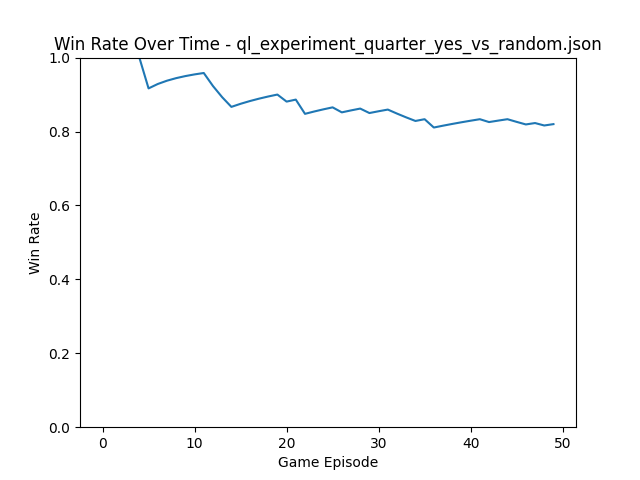
\includegraphics[width=0.25\textwidth]{images/win_rate_ql_experiment_quarter_yes_vs_random.png} &
    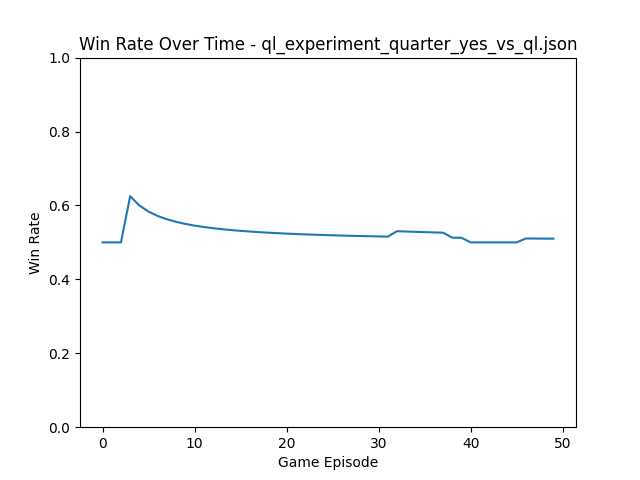
\includegraphics[width=0.25\textwidth]{images/win_rate_ql_experiment_quarter_yes_vs_ql.png} &
    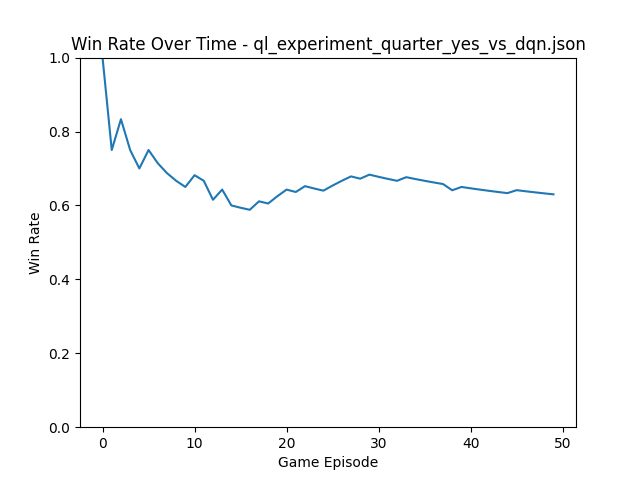
\includegraphics[width=0.25\textwidth]{images/win_rate_ql_experiment_quarter_yes_vs_dqn.png} \\
    \textbf{Second} & 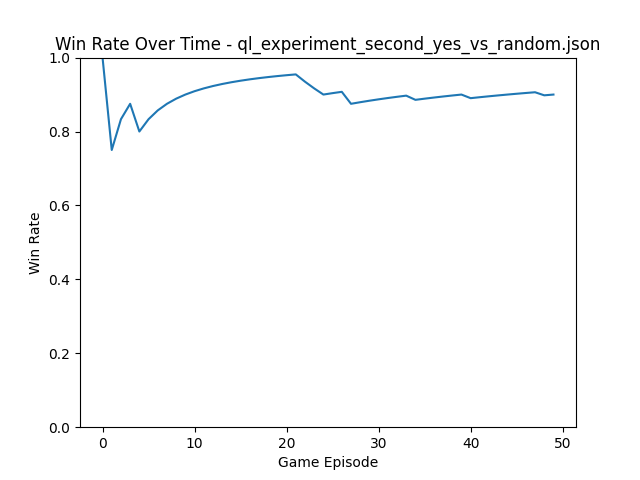
\includegraphics[width=0.25\textwidth]{images/win_rate_ql_experiment_second_yes_vs_random.png} &
    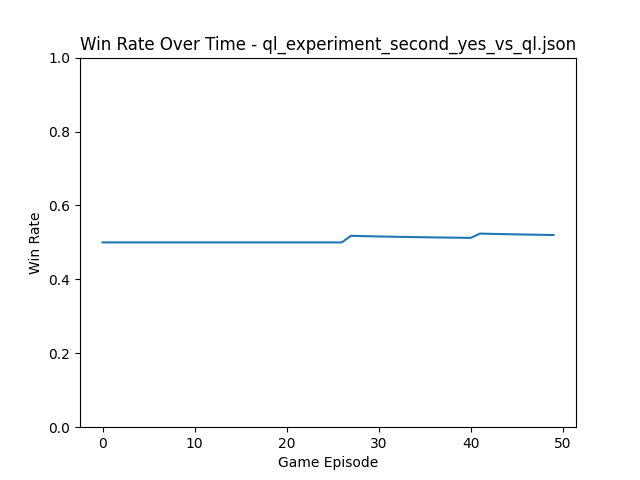
\includegraphics[width=0.25\textwidth]{images/win_rate_ql_experiment_second_yes_vs_ql.png} &
    \includegraphics[width=0.25\textwidth]{images/win_rate_ql_experiment_second_yes_vs_dqn.png} \\
  \end{tabular}


There were a plethora of interesting results in this experiment. From DQN having several promising experiments showing the capability of maintaining around the same win ratio with every opponent, to the exact same experiment but with QL instead of DQN falling
completely flat and not able to compete at all. For DQN, neutral, quarter, and half without alternating seemed to maintain nearly the same win ratio across all of the models but second seems to perform better against the random agent but worse against the 
other two. Adding alternating into the equation seems to have the trained agent perform slightly better then without it but still maintained a similar win rate sitting at 50-60 percent. This could enable further research on developing agents that have 
differing degrees of challenging so that players can decide how much they want their skill to be pushed.

As for QL, the only option that showed any promise in without alternating was the neutral option, though maybe that is to be expected with the simplistic model. Throw in alternating into the model, and it still performs much to well against a lesser skilled 
opponent, the random agent, but is able to hit that around 50 percent goal for the other two. Not the most promising results with this model but still valuable data and there are definitely shortcomings that can be expanded upon in this experiment. 

  \subsection{Improvements}

How could future work or research build upon this experiment and overcome the shortcomings? Well the first would be to expand the environment to more decisions. Starcraft II for example has no shortage of those, the environment would simply need to have 
other possible actions and states added. Then the experiment could truly thrive when instead of 21 states and 6 actions, there could be thousands of states and hundreds of actions, depending on how far further research goes, as there are plenty more 
states and actions in this environment as discussed in a previous section. 

Secondly, better models. Both of these trained models, QL and DQN, are at the end of the day simplistic and not the end goal. Previous research mentioned have improved models that are trained on replays rather then just learning as they play, trained on 
multiple gpus rather then a single, consumer grade gpu, and trained over the course of weeks instead of days. This research in combination with those excellent papers and codebase seen before would induce a sophisticate experiment that will expand upon 
what was discovered here and give results that not just Starcraft II can do, but any games leading to possibly completely novel experience in games that has not been implemented yet. These improvements would be a few options of a path forward.
\section{Future Research}
\label{sec:future}


Based on the results of the experiment leaves room for both promise, and plenty of future work. Plenty of these results showed that there can be success, and the measure of success being close to a 50 percent win ratio, with this approach, however this model
is simplistic even if it already shows promise.

Work to be done in the future on this research would firstly be, a more complicated environment and model space specifically for Starcraft II, but even further then that, a multitude of games. In theory, if it works in a game like Starcraft II with actions and 
environment states on an increasingly high level, it should also be applicable to other games. Using other models research that was mentioned here\cite{starcraft_unplugged}\cite{liu2021mAS}\cite{liu2021mASreport}\cite{vinyals2017starcraft}, and many more as the 
research in creating a near perfect skilled model in a video games, like Starcraft II, has been thoroughly and expertly researched. Exploiting that research and combining this with more computation capabilities and time into the problem would lead to a potential
agent whose skill truly could compete with any level and not just a few basic models. 

Along with that, further research could be done in making the skill level alternate, for example one out of ever three actions could be the best, or fluctuating between half best, second best, and so on. Other methodologies on how to fluctuate skill could also 
be researched and tested  as this was simple a proof of concept and first go around of testing a complicated environment with the intention of making a model not perfect all the time, but the novelty being changing its skill level which was proving partially true
capable of doing so in a simple setting. 

Further research in developing an agent that players can select the level of challenge, for example neutral without alternating above in the DQN, managed around a 40 percent win ratio against each opponent. So if a player wanted a more relaxed but not easy gameplay
this would be a good difficulty setting to apply, adding further novelty to this idea with not only scaling difficulties, but indeed the capability to determine how challenging a model can be based on the players skill. 
\section{Conclusion}
\label{sec:conclusion}


To bring this research to a close, what was accomplished in this experiment was a novel idea to make a reinforcement learning agent in a video game with a complicated environment, in this case Starcraft II, capable of competing with a difficult opponent provide a
challenge and winning in some cases, here with the best of the models it would still maintain a 50 percent win rate, but also dropping down to in skill to a less worthy opponent, like a random agent, and maintaining a 50 percent, or close, win ratio. 

This hypothesis showed promise in the fact that in several of the tests, such as alternating between best and half best, did reach near that goal over the course of 50 games against three opponents at nearly a 60 percent ratio, and with the non-alternating neutral 
the ratio was almost 40 percent. Meaning research could go even further for multiple degrees of competitive play. 

To test the hypothesis 3 agents were built, a random agent for training and pure random testing, a simple Q learning agent for a baseline as well as reliable results, and a DQN model. Each of these had their strengths and weaknesses but together applied a wide 
range of tests to experiment with the theory behind. Those tests were performed by the two trained agents against all three agents with 50 games per model state with competitive level and alternating level. 

To conclude, further research in this field is exciting and novel, which I hope to look into more as knowledge, computation, and time to spend on it increases. 
\newpage
\section{Acknowledgements}
\label{sec:Acknowledgements}

Just a few Acknowledgements to make. I would like to thank the authors of the cited references for showing environments that can be used for this experiment as well as the art of the possible. As well as my wife, family, and friends for supporting me in the research
found here.
\newpage

%REFRENCES
\titleformat{\section}{\normalfont\huge\bfseries}{\thesection}{1em}{} 
\newpage

\addcontentsline{toc}{section}{References} %Adds the reference to the Table of Contents
\bibliography{bibliography}
\newpage

%APPENDICES
\appendix
\setcounter{page}{1} %Restarts page counting to 1
\pagenumbering{roman} %Differentiates the appendix page numbers from the main article

\titleformat{\section}{\centering\normalfont\normalsize\bfseries}{Appendix \thesection: }{0em}{}
\newpage
\section{Tables}
\renewcommand{\thetable}{\thesection \arabic{table}}
\setcounter{table}{0}

\includegraphics[width=0.5\textwidth]{images/cumulative_reward_dqn_experiment_half_no_vs_dqn.png} 
\includegraphics[width=0.5\textwidth]{images/cumulative_reward_dqn_experiment_half_no_vs_ql.png} 
\includegraphics[width=0.5\textwidth]{images/cumulative_reward_dqn_experiment_half_no_vs_random.png} 
\includegraphics[width=0.5\textwidth]{images/cumulative_reward_dqn_experiment_half_yes_vs_dqn.png} 
\includegraphics[width=0.5\textwidth]{images/cumulative_reward_dqn_experiment_half_yes_vs_ql.png} 
\includegraphics[width=0.5\textwidth]{images/cumulative_reward_dqn_experiment_half_yes_vs_random.png} 
\includegraphics[width=0.5\textwidth]{images/cumulative_reward_dqn_experiment_neutral_no_vs_dqn.png} 
\includegraphics[width=0.5\textwidth]{images/cumulative_reward_dqn_experiment_neutral_no_vs_ql.png} 
\includegraphics[width=0.5\textwidth]{images/cumulative_reward_dqn_experiment_neutral_no_vs_random.png} 
\includegraphics[width=0.5\textwidth]{images/cumulative_reward_dqn_experiment_neutral_yes_vs_dqn.png} 
\includegraphics[width=0.5\textwidth]{images/cumulative_reward_dqn_experiment_neutral_yes_vs_ql.png} 
\includegraphics[width=0.5\textwidth]{images/cumulative_reward_dqn_experiment_neutral_yes_vs_random.png} 
\includegraphics[width=0.5\textwidth]{images/cumulative_reward_dqn_experiment_none_none_vs_ql.png} 
\includegraphics[width=0.5\textwidth]{images/cumulative_reward_dqn_experiment_quarter_no_vs_dqn.png} 
\includegraphics[width=0.5\textwidth]{images/cumulative_reward_dqn_experiment_quarter_no_vs_ql.png} 
\includegraphics[width=0.5\textwidth]{images/cumulative_reward_dqn_experiment_quarter_no_vs_random.png} 
\includegraphics[width=0.5\textwidth]{images/cumulative_reward_dqn_experiment_quarter_yes_vs_dqn.png} 
\includegraphics[width=0.5\textwidth]{images/cumulative_reward_dqn_experiment_quarter_yes_vs_ql.png} 
\includegraphics[width=0.5\textwidth]{images/cumulative_reward_dqn_experiment_quarter_yes_vs_random.png} 
\includegraphics[width=0.5\textwidth]{images/cumulative_reward_dqn_experiment_second_no_vs_dqn.png} 
\includegraphics[width=0.5\textwidth]{images/cumulative_reward_dqn_experiment_second_no_vs_ql.png} 
\includegraphics[width=0.5\textwidth]{images/cumulative_reward_dqn_experiment_second_no_vs_random.png} 
\includegraphics[width=0.5\textwidth]{images/cumulative_reward_dqn_experiment_second_yes_vs_dqn.png} 
\includegraphics[width=0.5\textwidth]{images/cumulative_reward_dqn_experiment_second_yes_vs_ql.png} 
\includegraphics[width=0.5\textwidth]{images/cumulative_reward_dqn_experiment_second_yes_vs_random.png} 
\includegraphics[width=0.5\textwidth]{images/cumulative_reward_ql_experiment_half_no_vs_dqn.png} 
\includegraphics[width=0.5\textwidth]{images/cumulative_reward_ql_experiment_half_no_vs_ql.png} 
\includegraphics[width=0.5\textwidth]{images/cumulative_reward_ql_experiment_half_no_vs_random.png} 
\includegraphics[width=0.5\textwidth]{images/cumulative_reward_ql_experiment_half_yes_vs_dqn.png} 
\includegraphics[width=0.5\textwidth]{images/cumulative_reward_ql_experiment_half_yes_vs_ql.png} 
\includegraphics[width=0.5\textwidth]{images/cumulative_reward_ql_experiment_half_yes_vs_random.png} 
\includegraphics[width=0.5\textwidth]{images/cumulative_reward_ql_experiment_neutral_no_vs_dqn.png} 
\includegraphics[width=0.5\textwidth]{images/cumulative_reward_ql_experiment_neutral_no_vs_ql.png} 
\includegraphics[width=0.5\textwidth]{images/cumulative_reward_ql_experiment_neutral_no_vs_random.png} 
\includegraphics[width=0.5\textwidth]{images/cumulative_reward_ql_experiment_neutral_yes_vs_dqn.png} 
\includegraphics[width=0.5\textwidth]{images/cumulative_reward_ql_experiment_neutral_yes_vs_ql.png} 
\includegraphics[width=0.5\textwidth]{images/cumulative_reward_ql_experiment_neutral_yes_vs_random.png} 
\includegraphics[width=0.5\textwidth]{images/cumulative_reward_ql_experiment_quarter_no_vs_dqn.png} 
\includegraphics[width=0.5\textwidth]{images/cumulative_reward_ql_experiment_quarter_no_vs_ql.png} 
\includegraphics[width=0.5\textwidth]{images/cumulative_reward_ql_experiment_quarter_no_vs_random.png} 
\includegraphics[width=0.5\textwidth]{images/cumulative_reward_ql_experiment_quarter_yes_vs_dqn.png} 
\includegraphics[width=0.5\textwidth]{images/cumulative_reward_ql_experiment_quarter_yes_vs_ql.png} 
\includegraphics[width=0.5\textwidth]{images/cumulative_reward_ql_experiment_quarter_yes_vs_random.png} 
\includegraphics[width=0.5\textwidth]{images/cumulative_reward_ql_experiment_second_no_vs_dqn.png} 
\includegraphics[width=0.5\textwidth]{images/cumulative_reward_ql_experiment_second_no_vs_ql.png} 
\includegraphics[width=0.5\textwidth]{images/cumulative_reward_ql_experiment_second_no_vs_random.png} 
\includegraphics[width=0.5\textwidth]{images/cumulative_reward_ql_experiment_second_yes_vs_dqn.png} 
\includegraphics[width=0.5\textwidth]{images/cumulative_reward_ql_experiment_second_yes_vs_ql.png} 
\includegraphics[width=0.5\textwidth]{images/cumulative_reward_ql_experiment_second_yes_vs_random.png} 
\includegraphics[width=0.5\textwidth]{images/moving_average_reward_dqn_experiment_half_no_vs_dqn.png} 
\includegraphics[width=0.5\textwidth]{images/moving_average_reward_dqn_experiment_half_no_vs_ql.png} 
\includegraphics[width=0.5\textwidth]{images/moving_average_reward_dqn_experiment_half_no_vs_random.png} 
\includegraphics[width=0.5\textwidth]{images/moving_average_reward_dqn_experiment_half_yes_vs_dqn.png} 
\includegraphics[width=0.5\textwidth]{images/moving_average_reward_dqn_experiment_half_yes_vs_ql.png} 
\includegraphics[width=0.5\textwidth]{images/moving_average_reward_dqn_experiment_half_yes_vs_random.png} 
\includegraphics[width=0.5\textwidth]{images/moving_average_reward_dqn_experiment_neutral_no_vs_dqn.png} 
\includegraphics[width=0.5\textwidth]{images/moving_average_reward_dqn_experiment_neutral_no_vs_ql.png} 
\includegraphics[width=0.5\textwidth]{images/moving_average_reward_dqn_experiment_neutral_no_vs_random.png} 
\includegraphics[width=0.5\textwidth]{images/moving_average_reward_dqn_experiment_neutral_yes_vs_dqn.png} 
\includegraphics[width=0.5\textwidth]{images/moving_average_reward_dqn_experiment_neutral_yes_vs_ql.png} 
\includegraphics[width=0.5\textwidth]{images/moving_average_reward_dqn_experiment_neutral_yes_vs_random.png} 
\includegraphics[width=0.5\textwidth]{images/moving_average_reward_dqn_experiment_none_none_vs_ql.png} 
\includegraphics[width=0.5\textwidth]{images/moving_average_reward_dqn_experiment_quarter_no_vs_dqn.png} 
\includegraphics[width=0.5\textwidth]{images/moving_average_reward_dqn_experiment_quarter_no_vs_ql.png} 
\includegraphics[width=0.5\textwidth]{images/moving_average_reward_dqn_experiment_quarter_no_vs_random.png} 
\includegraphics[width=0.5\textwidth]{images/moving_average_reward_dqn_experiment_quarter_yes_vs_dqn.png} 
\includegraphics[width=0.5\textwidth]{images/moving_average_reward_dqn_experiment_quarter_yes_vs_ql.png} 
\includegraphics[width=0.5\textwidth]{images/moving_average_reward_dqn_experiment_quarter_yes_vs_random.png} 
\includegraphics[width=0.5\textwidth]{images/moving_average_reward_dqn_experiment_second_no_vs_dqn.png} 
\includegraphics[width=0.5\textwidth]{images/moving_average_reward_dqn_experiment_second_no_vs_ql.png} 
\includegraphics[width=0.5\textwidth]{images/moving_average_reward_dqn_experiment_second_no_vs_random.png} 
\includegraphics[width=0.5\textwidth]{images/moving_average_reward_dqn_experiment_second_yes_vs_dqn.png} 
\includegraphics[width=0.5\textwidth]{images/moving_average_reward_dqn_experiment_second_yes_vs_ql.png} 
\includegraphics[width=0.5\textwidth]{images/moving_average_reward_dqn_experiment_second_yes_vs_random.png} 
\includegraphics[width=0.5\textwidth]{images/moving_average_reward_ql_experiment_half_no_vs_dqn.png} 
\includegraphics[width=0.5\textwidth]{images/moving_average_reward_ql_experiment_half_no_vs_ql.png} 
\includegraphics[width=0.5\textwidth]{images/moving_average_reward_ql_experiment_half_no_vs_random.png} 
\includegraphics[width=0.5\textwidth]{images/moving_average_reward_ql_experiment_half_yes_vs_dqn.png} 
\includegraphics[width=0.5\textwidth]{images/moving_average_reward_ql_experiment_half_yes_vs_ql.png} 
\includegraphics[width=0.5\textwidth]{images/moving_average_reward_ql_experiment_half_yes_vs_random.png} 
\includegraphics[width=0.5\textwidth]{images/moving_average_reward_ql_experiment_neutral_no_vs_dqn.png} 
\includegraphics[width=0.5\textwidth]{images/moving_average_reward_ql_experiment_neutral_no_vs_ql.png} 
\includegraphics[width=0.5\textwidth]{images/moving_average_reward_ql_experiment_neutral_no_vs_random.png} 
\includegraphics[width=0.5\textwidth]{images/moving_average_reward_ql_experiment_neutral_yes_vs_dqn.png} 
\includegraphics[width=0.5\textwidth]{images/moving_average_reward_ql_experiment_neutral_yes_vs_ql.png} 
\includegraphics[width=0.5\textwidth]{images/moving_average_reward_ql_experiment_neutral_yes_vs_random.png} 
\includegraphics[width=0.5\textwidth]{images/moving_average_reward_ql_experiment_quarter_no_vs_dqn.png} 
\includegraphics[width=0.5\textwidth]{images/moving_average_reward_ql_experiment_quarter_no_vs_ql.png} 
\includegraphics[width=0.5\textwidth]{images/moving_average_reward_ql_experiment_quarter_no_vs_random.png} 
\includegraphics[width=0.5\textwidth]{images/moving_average_reward_ql_experiment_quarter_yes_vs_dqn.png} 
\includegraphics[width=0.5\textwidth]{images/moving_average_reward_ql_experiment_quarter_yes_vs_ql.png} 
\includegraphics[width=0.5\textwidth]{images/moving_average_reward_ql_experiment_quarter_yes_vs_random.png} 
\includegraphics[width=0.5\textwidth]{images/moving_average_reward_ql_experiment_second_no_vs_dqn.png} 
\includegraphics[width=0.5\textwidth]{images/moving_average_reward_ql_experiment_second_no_vs_ql.png} 
\includegraphics[width=0.5\textwidth]{images/moving_average_reward_ql_experiment_second_no_vs_random.png} 
\includegraphics[width=0.5\textwidth]{images/moving_average_reward_ql_experiment_second_yes_vs_dqn.png} 
\includegraphics[width=0.5\textwidth]{images/moving_average_reward_ql_experiment_second_yes_vs_ql.png} 
\includegraphics[width=0.5\textwidth]{images/moving_average_reward_ql_experiment_second_yes_vs_random.png} 
\includegraphics[width=0.5\textwidth]{images/win_rate_dqn_experiment_half_no_vs_dqn.png} 
\includegraphics[width=0.5\textwidth]{images/win_rate_dqn_experiment_half_no_vs_ql.png} 
\includegraphics[width=0.5\textwidth]{images/win_rate_dqn_experiment_half_no_vs_random.png} 
\includegraphics[width=0.5\textwidth]{images/win_rate_dqn_experiment_half_yes_vs_dqn.png} 
\includegraphics[width=0.5\textwidth]{images/win_rate_dqn_experiment_half_yes_vs_ql.png} 
\includegraphics[width=0.5\textwidth]{images/win_rate_dqn_experiment_half_yes_vs_random.png} 
\includegraphics[width=0.5\textwidth]{images/win_rate_dqn_experiment_neutral_no_vs_dqn.png} 
\includegraphics[width=0.5\textwidth]{images/win_rate_dqn_experiment_neutral_no_vs_ql.png} 
\includegraphics[width=0.5\textwidth]{images/win_rate_dqn_experiment_neutral_no_vs_random.png} 
\includegraphics[width=0.5\textwidth]{images/win_rate_dqn_experiment_neutral_yes_vs_dqn.png} 
\includegraphics[width=0.5\textwidth]{images/win_rate_dqn_experiment_neutral_yes_vs_ql.png} 
\includegraphics[width=0.5\textwidth]{images/win_rate_dqn_experiment_neutral_yes_vs_random.png} 
\includegraphics[width=0.5\textwidth]{images/win_rate_dqn_experiment_none_none_vs_ql.png} 
\includegraphics[width=0.5\textwidth]{images/win_rate_dqn_experiment_quarter_no_vs_dqn.png} 
\includegraphics[width=0.5\textwidth]{images/win_rate_dqn_experiment_quarter_no_vs_ql.png} 
\includegraphics[width=0.5\textwidth]{images/win_rate_dqn_experiment_quarter_no_vs_random.png} 
\includegraphics[width=0.5\textwidth]{images/win_rate_dqn_experiment_quarter_yes_vs_dqn.png} 
\includegraphics[width=0.5\textwidth]{images/win_rate_dqn_experiment_quarter_yes_vs_ql.png} 
\includegraphics[width=0.5\textwidth]{images/win_rate_dqn_experiment_quarter_yes_vs_random.png} 
\includegraphics[width=0.5\textwidth]{images/win_rate_dqn_experiment_second_no_vs_dqn.png} 
\includegraphics[width=0.5\textwidth]{images/win_rate_dqn_experiment_second_no_vs_ql.png} 
\includegraphics[width=0.5\textwidth]{images/win_rate_dqn_experiment_second_no_vs_random.png} 
\includegraphics[width=0.5\textwidth]{images/win_rate_dqn_experiment_second_yes_vs_dqn.png} 
\includegraphics[width=0.5\textwidth]{images/win_rate_dqn_experiment_second_yes_vs_ql.png} 
\includegraphics[width=0.5\textwidth]{images/win_rate_dqn_experiment_second_yes_vs_random.png} 
\includegraphics[width=0.5\textwidth]{images/win_rate_ql_experiment_half_no_vs_dqn.png} 
\includegraphics[width=0.5\textwidth]{images/win_rate_ql_experiment_half_no_vs_ql.png} 
\includegraphics[width=0.5\textwidth]{images/win_rate_ql_experiment_half_no_vs_random.png} 
\includegraphics[width=0.5\textwidth]{images/win_rate_ql_experiment_half_yes_vs_dqn.png} 
\includegraphics[width=0.5\textwidth]{images/win_rate_ql_experiment_half_yes_vs_ql.png} 
\includegraphics[width=0.5\textwidth]{images/win_rate_ql_experiment_half_yes_vs_random.png} 
\includegraphics[width=0.5\textwidth]{images/win_rate_ql_experiment_neutral_no_vs_dqn.png} 
\includegraphics[width=0.5\textwidth]{images/win_rate_ql_experiment_neutral_no_vs_ql.png} 
\includegraphics[width=0.5\textwidth]{images/win_rate_ql_experiment_neutral_no_vs_random.png} 
\includegraphics[width=0.5\textwidth]{images/win_rate_ql_experiment_neutral_yes_vs_dqn.png} 
\includegraphics[width=0.5\textwidth]{images/win_rate_ql_experiment_neutral_yes_vs_ql.png} 
\includegraphics[width=0.5\textwidth]{images/win_rate_ql_experiment_neutral_yes_vs_random.png} 
\includegraphics[width=0.5\textwidth]{images/win_rate_ql_experiment_quarter_no_vs_dqn.png} 
\includegraphics[width=0.5\textwidth]{images/win_rate_ql_experiment_quarter_no_vs_ql.png} 
\includegraphics[width=0.5\textwidth]{images/win_rate_ql_experiment_quarter_no_vs_random.png} 
\includegraphics[width=0.5\textwidth]{images/win_rate_ql_experiment_quarter_yes_vs_dqn.png} 
\includegraphics[width=0.5\textwidth]{images/win_rate_ql_experiment_quarter_yes_vs_ql.png} 
\includegraphics[width=0.5\textwidth]{images/win_rate_ql_experiment_quarter_yes_vs_random.png} 
\includegraphics[width=0.5\textwidth]{images/win_rate_ql_experiment_second_no_vs_dqn.png} 
\includegraphics[width=0.5\textwidth]{images/win_rate_ql_experiment_second_no_vs_ql.png} 
\includegraphics[width=0.5\textwidth]{images/win_rate_ql_experiment_second_no_vs_random.png} 
\includegraphics[width=0.5\textwidth]{images/win_rate_ql_experiment_second_yes_vs_dqn.png} 
\includegraphics[width=0.5\textwidth]{images/win_rate_ql_experiment_second_yes_vs_ql.png} 
\includegraphics[width=0.5\textwidth]{images/win_rate_ql_experiment_second_yes_vs_random.png} 


\end{document}
